\paragraph{abbot} the head \s{monk} of a \s{monastery}. Often addressed as “father” or “mother”. 
\paragraph{abuse of powers} the religious \s{crime} of abusing the powers of a priest. This includes the powers of the synod, as well as liao ceremonies.
\paragraph{Alderly} a forested region in central \s{Mournwold}, held by the \s{jotun}.
\paragraph{aldermen} a representative of a \s{market town}. In most cases these men or women are wealthy merchants of the town, but often they include prominent town folk such as a \s{friar} or blacksmith who lives in the village. Those market towns that employ their own militia usually raise the captain to the rank of alderman. The innkeeper is almost invariably an alderman of the town and can be one of the wealthiest members of the community. Many aldermen take great pride in their ceremonial chains of office. Several towns are in competition in providing the most magnificent chain for their representative, and some go so far as to commission them as \s{magickal item}s, such as an Alderman's Edge. \proverb{Without labour nothing prospers.}
\paragraph{ambergelt} a resin in red or similar colours, generally symbolised by a wasp. Used by \s{magicksmith}s to create \s{magickal item}s that heal, slow or preserve life. Also used for decoration, or as a resinous varnish.
\paragraph{Ambition} a \s{virtue} \proverb{There's never a tree so big it can't be felled.}
\paragraph{amity} (do not confuse with \s{enmity}) means that an \s{eternal} and their \s{herald}s are considered to be \s{foreigner}s, and therefore have the same protection under the \s{law} as Imperial \s{citizen}s.
\paragraph{anoint} a priestly ceremony strengthening the immediate connection between an individual and a \s{virtue} for short time.
\paragraph{Anvil} location of the \s{sentinel gate} and the \s{senate} and capital location of the \s{Empire}. Four times a year the powerful citizens of the \s{Empire} meet here to determine the future of their people. Founded on the ruins of the old smithy in which the \s{first Empress} took shelter from her enemies when a young woman, Anvil is said to be where the first open declaration of the dream of \s{Empire} was made. \localpar After her ascension to the throne, the Empress declared that the small settlement would be preserved for the lifetime of the \s{Empire} in memory of sacrifices made by those sheltering her. Since then Imperial parliaments have been held there, but the town itself has never been allowed to grow. In addition to the senate and sentinel gate, Anvil's permanent features are the Forge (now a pub), the Imperial \s{regio} and the site of the war memorial.%Tyke's eatery (\emph{Dine at Tyke's!}) 
\paragraph{Applewood} a village in \s{Stock March}, founded by a coalition of several \s{household}s after a particularly vicious \s{Feni} attack in the 370s.
\paragraph{artisan's oil} an oleaginous goop used by \s{magicksmith}s to mend the structure of broken \s{magickal item}s.
\paragraph{artisan} a skilled craft worker who makes or creates things by hand that may be functional or strictly decorative. Often used synonymously with \s{magicksmith}.
\paragraph{Ashbrook} a region and eponymous river in \s{Upwold}.
\paragraph{assembly} the individual bodies of the \s{synod} are referred to as assemblies. The Marcher assembly, and most \s{virtue} assemblies, welcome interested laypeople such as \s{pilgrim}s of the way, friars, or priests without a congregation, even though these individuals do not have the right to vote on judgements.
\paragraph{autumn} 1: a season 2: the \s{magick}al realm of wealth, bargins and power \proverb{Reap what you sow, come rain, shine or snow.}
\bigparagraph{bailiff of the grand market} The bailiff of the grand market is an Imperial title awarded to a Marcher citizen. It is a Marcher position appointed through the Bourse but chosen by Marcher yeomen with votes allocated based on the size of their farm holdings. The bailiff has offices in Meade, but it is a rare bailiff who spends much time there. While the title is associated closely with the weekly or bi-weekly markets of Mitwold, the bailiff is regularly involved in trade fairs and markets across the Marches, and Marchers from every territory have regularly held the post. \localpar The title pre-dates the formation of the \s{market town}s, and comes from a time when almost every town and village in the nation would have their own regular market. Traditionally the bailiff's role was to ensure security at fairs and markets across the Marches. In return, they were guaranteed a hearty meal, a minimum of one meat pie and a tankard of ale. \localpar More importantly, however, to help the bailiff meet the costs of their office they were given the opportunity to buy some goods before the market officially opened, allowing shrewd bailiffs to secure bargains for themselves. Many markets considered it a matter of Pride to ensure that the bailiff turned a good profit in exchange for their hard work in keeping the marketplace safe and fair for all. Within the space of a season, the bailiff might find themselves in a position to buy beggar's lye and ambergelt at a fair from a village in the birchwoods of \s{Upwold}; a cask of Wintermark mead and some measures of \s{dragonbone} from a Suaq peddlar in a town square in \s{Mitwold}; a basket of tempest jade from a scowling stallholder at the great market in Meade; a basket of assorted herbs at a dour fair in \s{Bregasland} or even a handful of \s{crystal mana} at a strained gathering in Overton. \localpar When the Marches joined the \s{Empire} some of the more expensive responsibilities of the bailiff were assumed by the civil service. Marchers are loath to abandon their traditions however; the presence of an honest bailiff was considered to be good for trade as it let everyone ken that the market was safe to travel to. With the help of Emperor Giovanni the role of bailiff was incorporated into the Bourse, to allow the \s{civil service} to identify the individual with the most support from other yeomen. \localpar The bailiff is expected to ensure fairs, markets and trade gatherings in the Marches are undertaken in a traditional and honest fashion. They also have some responsibility for ensuring that the major roads between towns and villages remain free of bandits and \s{Feni} who might otherwise restrict trade. In practice, this is quite a tall order for a single individual—many markets have their own local bailiff or sheriff who sees to the security of their fair. Specifically, the bailiff oversees the grand market in Meade which takes place on the third weekend of each month and attracts traders from across the Marches and even occasionally from Wintermark to the north. 
\paragraph{band} a \s{group} of citizens from the same \s{nation} bound together by magick and a common oath. Either a \s{banner} or a \s{sect} or a \s{coven}.
\paragraph{banner} a \s{band} of yeomen or other fighters fighting under a common oath and standart in war. Often, a Marcher \s{household} form a banner to fight under. Each citizen can be a member of only one banner, swearing in to a new banner breaks the bond to the old one. \proverb{Pride in the farm, Loyalty to those who tend it. Proud of the farm, loyal to the family. – House Greyshanks}
\paragraph{barbarian} anyone with whom the \s{Empire} is at war, including during a ceasefire. \s{eternal}s and the \s{herald}s of \s{eternal}s who are the subject of a declaration of \s{enmity} by the \s{conclave} are considered enemies of the \s{Empire} and treated as barbarians. Unauthorised dealings with barbarians are illegal and will be investigated as treason. Any delegations from barbarian nations who arrive on the field of Anvil under a flag of peace have protection under the \s{law} as if they were Imperial citizens for the duration of their visit and for their direct passage out of the \s{Empire}. Otherwise barbarians have no protection under the law.\proverb{Where the hedge is lowest men jump over.}
\paragraph{battle} a fight between many people on each side. In \s{Anvil}, \s{constellation}s usually permit two battles per week facilitated through the \s{sentinel gate}, involving fighters from five \s{nation}s to pass through the gate.
\paragraph{beak} the hard mouth of a bird or herald of \s{Lashonar}.
\paragraph{beater's gate} A wayhouse south of \s{Greywater}, kent for its hospitability, in particular to travelling \s{beater}s. The house was set up by Bobby Greyshanks (owner of \s{Bobby's bridge}) to provide accommodation for weary travellers.
\paragraph{beating the bounds} festival in autumn, after the gathering of harvest, when \s{beater}s lead the communities in remembering who and what is part of the community, or not. \proverb{Friends are the family we choose ourselves.}
\bigparagraph{beater} Beaters roam the Marches, learning every part of the land, watching for thieves, vagrants and other ne'er-do-wells. Beaters mark out what land belongs to whom.  Beaters are often instrumental in settling land disputes between neighbours and they still play a vital role in the tradition of the \s{beating of the bounds}. The beating of the bounds usually takes place after the harvest is in. At this festival every Marcher marks their land, by walking around the boundary led by the beaters. Certain stones, trees or other marker points around the boundary are beaten literally, ceremonially striking them with sticks or willow wands. The \s{market town}s beat the boundaries laid out by their warrant, and individual towners often have a second ceremony in which they beat the bounds of their shop or workplace. The ceremony is designed to remind all of the size of the holding, but it also works to remind everyone of who is part of the community and who is outside it. On a practical level, the beating of the bounds is often preceded by the beaters ensuring that the boundary areas are safe for the upcoming ceremony, and followed by a period of maintaining and replacing whatever physical markers delineate the bounds – it is a time for repairing fences, planting hedges and the like. Beaters often live off the land and most are skilled woodsmen and hunters. They serve as an informal police force, investigating crimes and tracking criminals. While an individual beater often associates with one or more \s{household}s, they make no secret of the fact that they maintain an informal network among themselves. The beaters watch the boundaries and defend them against trespass until its forces can muster. They also remain vigilant for internal threats. In addition to the orcs that still occupy the more inaccessible hills and wild forests of the Marches, there are bands of \s{Feni} who launch raids against civilised Marchers to steal metal, cattle or crops. If something or someone is raiding out of the forests or hills then the beaters are the ones who are called on to hunt it. The third Marcher army, the \s{bounders} of \s{Upwold}, contains a large number of beaters. \bigparagraphendtwiddle
\paragraph{becoming a Marcher} \see{march}
\paragraph{beggar's lye} a liquid solution produced from tree ash, generally symbolised by a skull. Used by magicksmiths as a caustic or primer that changes material properties in the process of creating \s{magickal item}s.
\paragraph{Birchland} a region in \s{Upwold}, fortified by the ancient \s{eastern guard}.
\paragraph{blasphemy} the religious \s{crime} of denigrating of the \s{paragon}s and the paths of \s{virtue}. This includes promoting false virtues and the teachings, or example, of false exemplars or false \s{paragon}s.
\paragraph{bleeding out} a serious \s{injury} can leave a soldier bleeding out, such that they will die after a few minutes (less if \s{poison}ed) unless saved by a healer of any competency.
\paragraph{Bobby's brigde} \see{Brock's toll}
\paragraph{boggart} a class of \s{vermin}, believed to have originated from the Realm of \s{night}. They vary from being cat-sized to about the size of a grown adult. Boggarts are manavores and deliberately seek out flows of magick, and the places they pool, to feed upon. Possessing an inherent magick akin to the \s{ritual} Twilight Masquerade, their primary defence is camouflage, and they rarely approach or attack citizens. Boggart feces are also kent to enrich – or perhaps transform – soils and enhance their fertility. Consequently, rarified boggart manure is sought after to enhance production of herb gardens or farms. The potency of these feces fades however swiftly. 
\paragraph{Bolstering Bill} or \keyword{Wilhelmina} \s{exemplar} of \s{Loyalty}. As a famous folk hero, many stories describe her exploits. She is usually depicted with her eponymous weapon, giving a hand to a comrade.\begin{figure} \centering 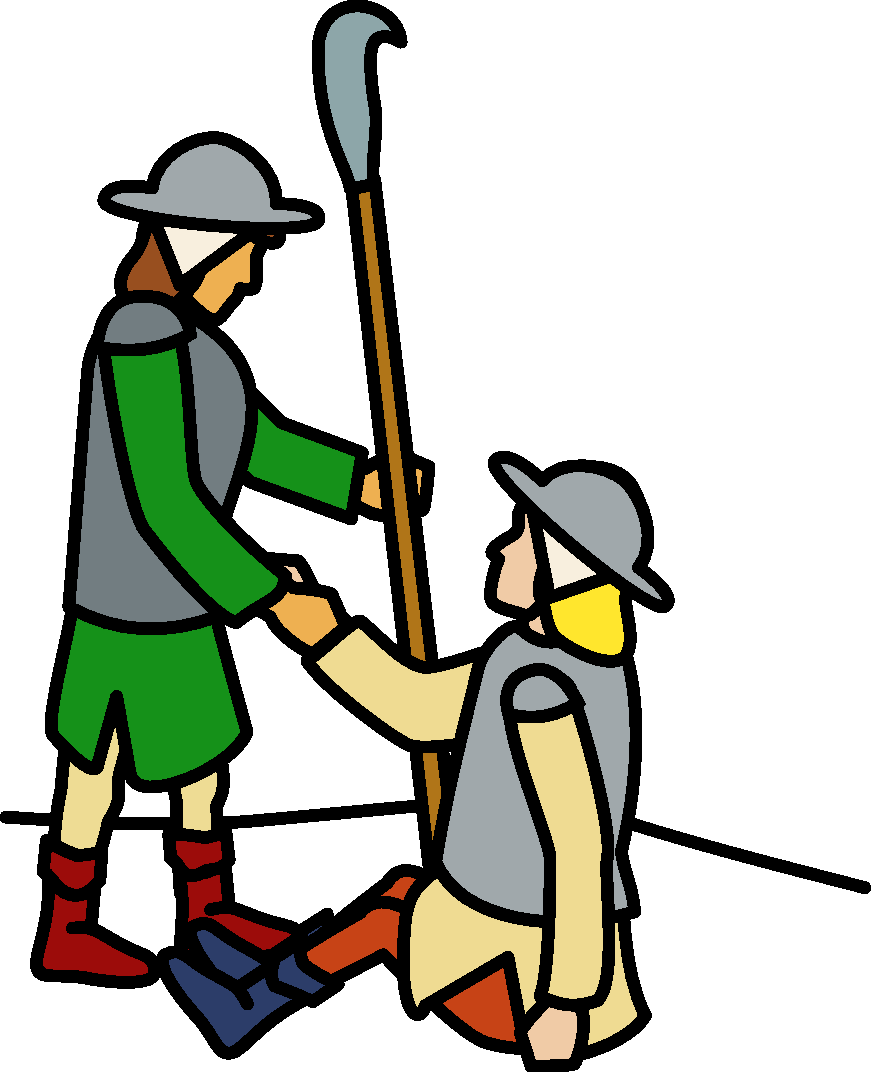
\includegraphics[width=5cm]{encyclopedia/Wilhelmina} \caption{Bolstering Bill*}\end{figure}
\paragraph{boundary dispute} when two Marchers both claim a piece of land, they should ask a wise \s{beater} from their region to settle the matter. If they cannot be settled, a sportive competition, such as games of tug-of-war, is a good matter to settle the dispute, once and for all or on a yearly cycle.
\paragraph{bounders} \keyword{1)} the third army of the Marches, made up from ruthless \s{Upwold} \s{yeomen}, \s{beater}s and \s{landskeeper}s \begin{figure}\centering
\includegraphics[width=5cm]{encyclopedia/TheBounders}\caption{Bounders emblem}\end{figure} 2) \keyword{Boundarymen}, a group of Upwold \s{beater}s, scouts and \s{yeomen} connected to the Bounders army, with the taken duty of keeping the land safe.
\paragraph{bourse} one of the great councils according to the \s{constitution}. The bourse is designed to ensure that \s{ilium}, \s{mithril}, \s{weirwood} and \s{white granite} are directed to where they can provide the most economic benefit, rather than being assigned by political or military patronage. Merchants bid for a position on the bourse and those that are successful gain control of one of the bourse positions that control production.\proverb{Nothing ventured, nothing gained.}
\paragraph{brass coast} a \s{nation} of the \s{Empire} where everything has a price in rings. An individual from the coast is a “freeborn”.
\paragraph{Bregasland} the westernmost of the Marches territories, comprising partially of fenland leading to the coast of \s{Westmere}. The territory is a place of small islands of abundantly fertile soil, surrounded by seemingly endless marshes where eels are caught. There are several \s{household}s here made up entirely of \s{merrow}, and several settlements populated by \s{shun}ned who cannot bring themselves to leave the Marches. Bregasland is home to partially sunken ruins, including several stone circles that pre-date Marcher possession of the land, and a variety of beasts and natural phenomena haunting the fens, such as \s{marshwalker}s, \s{willothe wisp}s, etc.
\paragraph{briar} a type of \s{lineaged}, touched by the \s{magick}al realm of \s{spring}. They mate and breed just like humans, they have hair, and they give birth to live offspring. Briars are almost never born expressing their lineage. Their lineage appears when they sustain a serious injury, with the site of the injury quickly covered in a thick scab with the texture and appearance of bark. Many people show no signs at all of being a briar before the bark appears. Once that happens, changes tend to happen quickly, thorns may appear growing through the skin and the eyes may turn green. The psychological effects of lineage appear at the same time. If a briar is wounded and healed with spring magick this can strengthen a briar's lineage; the physical and mental signs become more evident. \localpar After \s{death}, a briar’s entire body is slowly covered with bark, appearing a lot like a misshapen, fallen log. It is a common belief that a briar who avoids magickal healing will lose the taint of the blood and not pass it on to their offspring, although this is probably wishful thinking. An area where a briar is buried after \s{death} may be seeded with alien, supernatural foliage. Briars who got buried with vengeance or wrath can particularly affect the land with this taint, it is therefore recommended to bury dead briars in hedges or on islands surrounded by flowing water. In case of taint, it can often help to clearly delineate a boundary between the tainted land and the surroundings, and \s{beating of the bounds} between them, to keep the taint at bay.
\paragraph{Britta} “The Young Empress”, on the throne 374–376 YE. She died in \s{battle} against the \s{thule} at the autumn equinox 276, alongside large parts of the Empire's heros of her time.
\paragraph{Brock's toll} a famous toll bridge. The road that this bridge lies on carries most of the agricultural traffic between Dawn and the Marches, and the operator of the Toll is allowed by tradition to claim one sack from each carthe s load. The bridge is so old that when it was first constructed the Vallorn still controlled most of Miaren. \localpar In the early days of the \s{Empire} this site changed hands between the two \s{nation}s several times, often with violence. Even when Earls and Stewards forbade their people to fight, rowdy yeomen would often take matters into their own hands and the navarr soon became sick of breaking up scuffles over ownership. At some point the Imperial Senate took matters into their own hand and decreed that ownership of the Toll would be decided by an annual competition of arms between the yeomen who were so eager to fight. Eventually this evolved into the modern practice of Brock's Buffet—a brutal (nonlethal) five-aside melee each summer, with only one winner left standing to claim ownership for the coming year. The Buffet has traditionally been won by the Marches, and for its current owner, it is also kent as “Bobby Shanks' bridge”.
\paragraph{burial} rite after \s{death}. Marcher \s{hearth magick} requires that dead Marchers be buried in Marcher soil, to feed back into the cycle of \s{Prosperity}, often with an apple seed or small apple sapling planted above the body. There is some evidence that spirits of dead Marchers may trouble friends, relatives or even random travellers until their remains are given a suitable burial. In addition to the Marches themselves, there is an orchard in \s{holberg} that was turned into Marcher soil to bury a large number of dead Marchers that could not be brought home. \proverb{Sow, tend and reap; fight, toil and weep.}
\paragraph{calendar} we count the years since the foun\-da\-tion of the \s{Empire} (YE). The table lists the regular events in a year. \begin{table*}\centering \begin{tabular}{p{0.15\textwidth}p{0.8\textwidth}} date& event\\ \hline 1 jannery & New Year's Day \\ jannery & Clear ditches; cut wood; breed sows; spread manure; camping; early lambs \\ febbery & Prune grapes and fruit trees; prune and mend hedgerows; mend fences; kill moles; plant willow; add lime, chalk and manure to soil; lambing continues; calving begins \\ m' o'march & plow and harrow soft ground; sow spring grains; calving \\ early march & building the maiden at \s{Maidenstone} \\ 21 march & spring equinox summit in \s{Anvil}: selection of the general of the \s{tusks} army; auction of \s{ilium} \\ april & Plant onions and leeks; plant flax; wean calves; get milking and dairy work underway; farrowing (birth of piglets) \\ 1 may & Jack's birthday, according to \s{Bregasland} folklore \\ may & Weed winter corn; remove moss from thatched roofs and repair; sow pulses; capture swarming bees; mark sheep; plant beets, carrots, cabbages, and other garden vegetables \\ june & Wash and shear sheep; shear lambs later in the month; start mowing hay \\ 21 june & summer solstice summit in Anvil: the buffet for \s{Brock's toll}; election of the senator for \s{Mitwold}; selection of the general for the \s{drakes}; auction of \s{white granite}\\ july & mowing the hay; harvest flax and hemp; begin harvesting winter corn \\ august & Finish harvesting winter grain, begin on spring grain; gather in straw; plant turnips \\ september & Harvest peas; breed cattle; harvest honey; \s{beating of the bounds}; plow fields for winter grain; sow winter wheat and rye; harvest apples, blackberries; take excess stock to market; \s{wassail} \\ 21 september & autumn equinox festival in Anvil: election of the senator for \s{Upwold}; selection of the general for the \s{bounders} army; auction of \s{mithril} \\ october & Sow winter barley and oats; harvest grapes; make wine and verjuice; breed sheep; let pigs forage on acorns and beechnuts \\ 1 november & pooka's day \\ november & fatten swine; take in firewood; threshing and winnowing continue through the winter \\ december & Slaughter hogs; never too early to shovel manure \\ 21 december & winter solstice summit in Anvil: election of the \s{bailiff of the grand market}; election of the senator for \s{Bregasland}; selection of the general for the \s{strong reeds}; auction of \s{weirwood}; \s{return of the sun}\\ \hline 3rd weekend each month & grand market in Meade \end{tabular} \caption{calendar} \end{table*}
\paragraph{cellerar} the steward of a monastery, if the abbot is member of the synod
\paragraph{ceremony} the process of actualising a \s{virtue}, by creating an aura or manipulating a \s{citizen}'s \s{soul}. Performed by a priest using liao.
\paragraph{Chalk Downs} a chalky region in the northern \s{Mournwold}, held by the \s{jotun}.
\paragraph{chirurgeon} someone with basic training in \s{medicine}, able to stabilise someone to stop them from \s{bleeding out} from a mortal \s{injury}. \proverb{Healer's faults grow orchards.}
\paragraph{citizen} the \s{Empire}, according to its wise \s{constitution}, “recognize[s] as citizens those whose oath to accept the culture of a \s{nation}; to honour the \s{virtue}s of the way, and to support the \s{law}s of the \s{Empire}, is accepted by [an] egregore [such as \s{Jack-in-the-green}].” citizens are guaranteed “dignity, freedom, and Prosperity.” citizens must fulfil their obligations to the state and in return they receive associated rights, including protection under Imperial \s{law}. Individuals who have forsworn the oath to their egregore will be considered \s{foreigner}s, not \s{barbarian}s.
\paragraph{civil service} the members of the civil service, after long training in the Castle of Thorns in \s{Dawn}, are in charge of keeping the \s{Empire} running. Non-\s{magistrate} civil servants wear a golden \s{horse} head on purple.
\paragraph{clemency} a plea by a \s{priest} in a \s{trial} explaining the virtues and necessity of the crime.
\paragraph{conclave} the governing body for all \s{magick}al business in the \s{Empire}. It can eg. declare \s{amity} or \s{enmity} with \s{eternal}s, or officially declare someone a \s{sorcerer}.
\paragraph{consecrate} a priestly ceremony that allows a \s{monk} to put an aura of a \s{virtue} on a building.
\paragraph{constellation} a collection of stars and thus magickal symbol, map or chart of the powers of the world reflected above. \begin{table*}\centering \begin{tabular}{lp{0.35\textwidth}p{0.45\textwidth}} name& law& common magick\\ \hline the chain & things hold together & bonds, oaths \\ cup o'choices & things apart come together & healing, mending, connections \\ the claw & things bleed & battle, destruction, violence \\ the door & things move and change & transport, travel, personal change \\ the drowned man & things end & curses, misfortune, ending \\ the fountain & things live & growth, fertility, foundations \\ the great wyrm & things change and transform & magick, grand transformation \\ the key & things are revealed & scrying, opening, skills \\ the lock & things can be hidden & wards, defence, concealment \\ the mountain & things are not easy & obstacles, effort, trials \\ our good oak & things endure & strength, endurance, fortitude \\ the phoenix & things learn & ken \\ the spider & things are being watched & hidden forces, eternals, sovereigns \\ the stallion & things procreate & fertility, growth, wealth \\ the stork & things matter & decisions, responsibility, leadership \\ the web & things are connected & relationships, synchronicity, sympathy \\ the three sisters & things are connected by blood & consequences, ties of blood, sorrow \\ bloody crown & things are not what you think & destiny, fate, chance \end{tabular} \caption{constellations} \end{table*}
\paragraph{constitution} the fundamental law governing the rights and duties of all \s{citizen}s, giving fundamental tenets of, among other things, \s{senate}, \s{bourse} and \s{conclave}, \s{synod}, \s{military council}, \s{civil service} and the \s{throne}.
\paragraph{Courage} a \s{virtue}
\paragraph{coven} a \s{band} of magickians who join to cast \s{ritual}s together. A coven can only have members from a single \s{nation}, and the number of rituals they can cast together is limited, usually to two rituals per day. Each citizen can be a member of only one coven, swearing in to a new coven breaks the bond to the old one. A coven always shares an oath, and can have a covenstone to be more effective. \proverb{Serve the Marches, reap the rewards – The Reapers Coven}
\paragraph{crime}\s{law} Imperial \s{law} distinguishes between crimes against a person (eg. murder, or assault), crimes of property (eg. theft, or possession of \s{poison}s), crimes of position (eg. treason), crimes against the processes of the state (eg. subverting agencies of the state), and religious crimes (eg. \s{blasphemy}, or \s{heresy}). Civil claims are not crimes, but can still be heard by a magistrate in a \s{trial}. \proverb{What happens in the Marches stays in the Marches!}
\paragraph{cromlech}  a circle of \s{standing stone}s, often at a \s{regio}.
\paragraph{crown} 1: A piece of regal headgear. 2: A denomination of coins. One crown is worth 20 \s{ring}s, or $^1/_8$ of a \s{throne}. The annual tax for every \s{citizen} who owns a personal resource allocated by the \s{civil service} is one crown, according to the constitution.
\paragraph{crystal mana} \s{mana} in a form that allows it to be used for \s{ritual}s and spellcasting, generally not used for spellcasting. There are various forms of crystals, usually accompanied by a certificate.
\paragraph{curse} using magick on another person is never in and of itself a \s{crime}, but the \s{conclave} can declare offenders \s{sorcerer}s. Removing a curse is a significant indicating; rituals to remove a curse effect will almost always be many magnitudes higher than the magnitude of the ritual that created the curse. In most cases, a specific ritual or a minimum magnitude will be necessary. \localpar Each curse is unique, and the method of removing it also tends to be unique. The priestly ceremony of \s{insight} and the \s{ritual} bright lantern of ophis can help discern the nature of the curse and how to deal with it. Some curses can also be removed by the intervention of a powerful creature or item, such as the \s{eternal} \s{Ephisis}. Like rituals there is no single \s{eternal} with the power to remove just any curse, rather specific creatures or items have the ability to remove a specific curse. Powerful creatures almost invariably require quests or favours in return for removing a curse, and gaining their assistance or access to a powerful item are likely to involve difficult quests. \localpar Many curses in \s{Imperial lore} contain a pronouncement of doom, which makes it obvious to the target that they have been put under a curse. It is advisable to consult the Imperial lore about these. The following table contains an overview curses that are not delivered through such a pronouncement, or may require urgent reaction. \begin{table*}\centering \begin{tabular}{p{0.35\textwidth}p{0.18\textwidth}p{0.35\textwidth}} effect& cause& fix\\ \hline seeing only black and white& wraiths& exorcism\\ malignant spirits tormenting a territory, reduced production& winter's ghosts (w50)& wait 3 months\\ territory scoured with terrible thunderstorms& thunderous deluge (sp46)& wait 3 months\\ Madness, halucination, obsession& all the world in a grain of sand (d30) & transmogrification of the soul's echo (n60) \\ extremely strong emotions & unfettered anarchy (n10) & transmogrification of the soul's echo (n60)\\feeling feverish and unwell; skin constantly itches. Feeling as if under the effect of a \s{venom}, but the usual cures do not lend aid.& curse of gangrenous flesh (sp40)& certain powerful creatures or items; powerful rituals that remove curses of sickness such as the consumable produced by distill the serpenthe s stone.\\ feeling extremely aged and infirm, whatever the actual age. Feeling magickal \s{weakness}, but the usual cures do not lend aid.& curse of decrepitude (w50)& certain powerful creatures or items; powerful rituals that remove curses of sickness such as the consumable produced by distill the serpent's stone.\\ itching all over, biting insects & anathemic call of bug and briar (sp16) & some eternals \\ a growing chill and numbing throughout all the body, reduced movement, coma, reanimation as a flesh-hungry zombie bent on killing and devouring the living. & the moon’s \s{poison}& the balm called feast for the crows. The wrong antidote speeds up the process.\\ a growing heat spreading through the body, extremely short temper, voices urging them to kill everyone around.& the \s{poison} hunger of the wolf& the balm called feast for the crows. The wrong antidote speeds up the process. \end{tabular} \caption{common curses} \end{table*}
\paragraph{Dawn} nation west of the Marches. The Marches were formed by yeomen Marching in the rebel march out of dawn, carving their own place in the world. Marcher dislike of Dawn is a strong part of Marcher \s{hearth magick}, similar in nature to the rivalries between siblings, \s{household}s, territories, etc. within the nation. \proverb{Bread without spice is better than spice without bread.}
\paragraph{day} 1: a time 2: the \s{magick}al realm of spirit and ken
\paragraph{death} through old age, hunger, or through bleeding out if a mortal \s{injury} has been left untreated for too long, among other things, a man or woman can die. Their \s{soul} will then leave the body for the \s{labyrinth}, from whence it will return in due season. A \s{friar}, \s{monk} or other priest will ken the rites to help a dying Marcher hasten their way through the \s{labyrinth}. If at all possible, it is desirable that the dying Marcher be \s{shriven} before their soul leaves the body, so that they go to the labyrinth with fewer \s{sin}s, to return faster. In general, a Marcher should always be buried in Marcher soil, either under an existing apple tree or with the seeds for a new tree. Due to the \s{taint} that dead \s{briar}s can bring to the land, it is advisable to give these lineaged a resting place in \s{hedges} or on islands surrounded by flowing water instead. If no priest is at hand to say the rites for the burial, the congregation should speak of the \s{virtue}s of the dead, and say such \s{proverbs} as exemplify the turning of the circle.\proverb{Spring follows winter, dawn follows night, life follows death.}
\paragraph{declaration} a decision of the \s{conclave} %\proverb{Dine at Tyke's! You can eat anywhere.}
\paragraph{dedicate} for the average citizen of the \s{Empire}, it is simply enough to ken of the seven \s{virtue}s and how they apply to their lives. There is no requirement to honour one above another for all seven are part of the way and will guide their spirit through the labyrinth of ages. Priests of the way have made greater study of the mysteries and doctrines of the faith. They provide guidance to citizens about how to live virtuously and have learned ceremonies that enrich the lives of virtuous citizens and enhance an individual’s understanding of the \s{virtue}s. The liao ceremony of dedication allows a human to more sharply focus their spirit onto one particular virtue path. This focus enables a dedicated priest to perform other ceremonies that provide greater insight and illumination into the virtue. Consequently, dedication is reasonably common amongst priests who wish to provide ministry and guidance relating to a specific virtue, whilst other priests choose not to dedicate and so represent all seven virtues equally. While dedication does not aid reincarnation by itself, some layfolk do choose to become dedicated for their own reasons. Such individuals are called pilgrims. \proverb{Vows made in storms are forgotten in calms.}
\paragraph{desecration} the religious \s{crime} of removing spontaneously created auras such as legacies of ascendance to \s{paragon}hood. This includes such auras arising on areas, objects and people.
\paragraph{doctrine} the doctrines of the faith represent the correct understanding of the way. They have been debated, analysed and formally recognised by the synod. Teaching doctrines that are at odds with, and thus undermine, the doctrines of the faith is as heresy and thus a religious crime under the \s{law}.\begin{table*} \begin{tabular}{p{0.8\textwidth}}\emph{The Human Spirit is immortal}. It inhabits mortal flesh for a span within the world before being liberated again, having gained knowledge and enlightenment. It traverses the Labyrinth of Ages before returning to mortal life through new birth.\\ \emph{Only Human Spirits reincarnate}, therefore humans are the greatest of all beings in Creation for only human spirits gain strength, knowledge and enlightenment through rebirth. The Paragons not only personify Virtue but the full potential of humanity.\\\emph{There are Seven Virtues} that guide the spirit through the Labyrinth of Ages. These are Ambition, Courage, Loyalty, Pride, Prosperity, Vigilance and Wisdom. Other qualities may benefit humanity, but lend no aid through the passage of death to rebirth, and some may hinder it.\\\emph{A truly Virtuous Spirit, one who is a Paragon of Virtue}, is capable of freeing itself from the Labyrinth of Ages through transcendence. A Paragon Spirit can be identified for having completed at least six of the Eight Signs of the Paragon, after which it can be recognised by the Imperial Synod.\\\emph{Human destiny is our own}. The Creator Spirit, whose hand can be seen in all patterns of nature, seeks no dominance of, control over or communion with human spirits.\\\emph{The Labyrinth of Ages} is a place of pure spirit and beyond the true comprehension of any but a Paragon. Flesh and blood may not enter, only that which is of spirit may traverse into and out of it, and it has no peer.\end{tabular}\caption{the doctrines of the faith}\end{table*}
\paragraph{dolmen} a table made of two or more \s{standing stone}s with a slab on top \begin{figure}\centering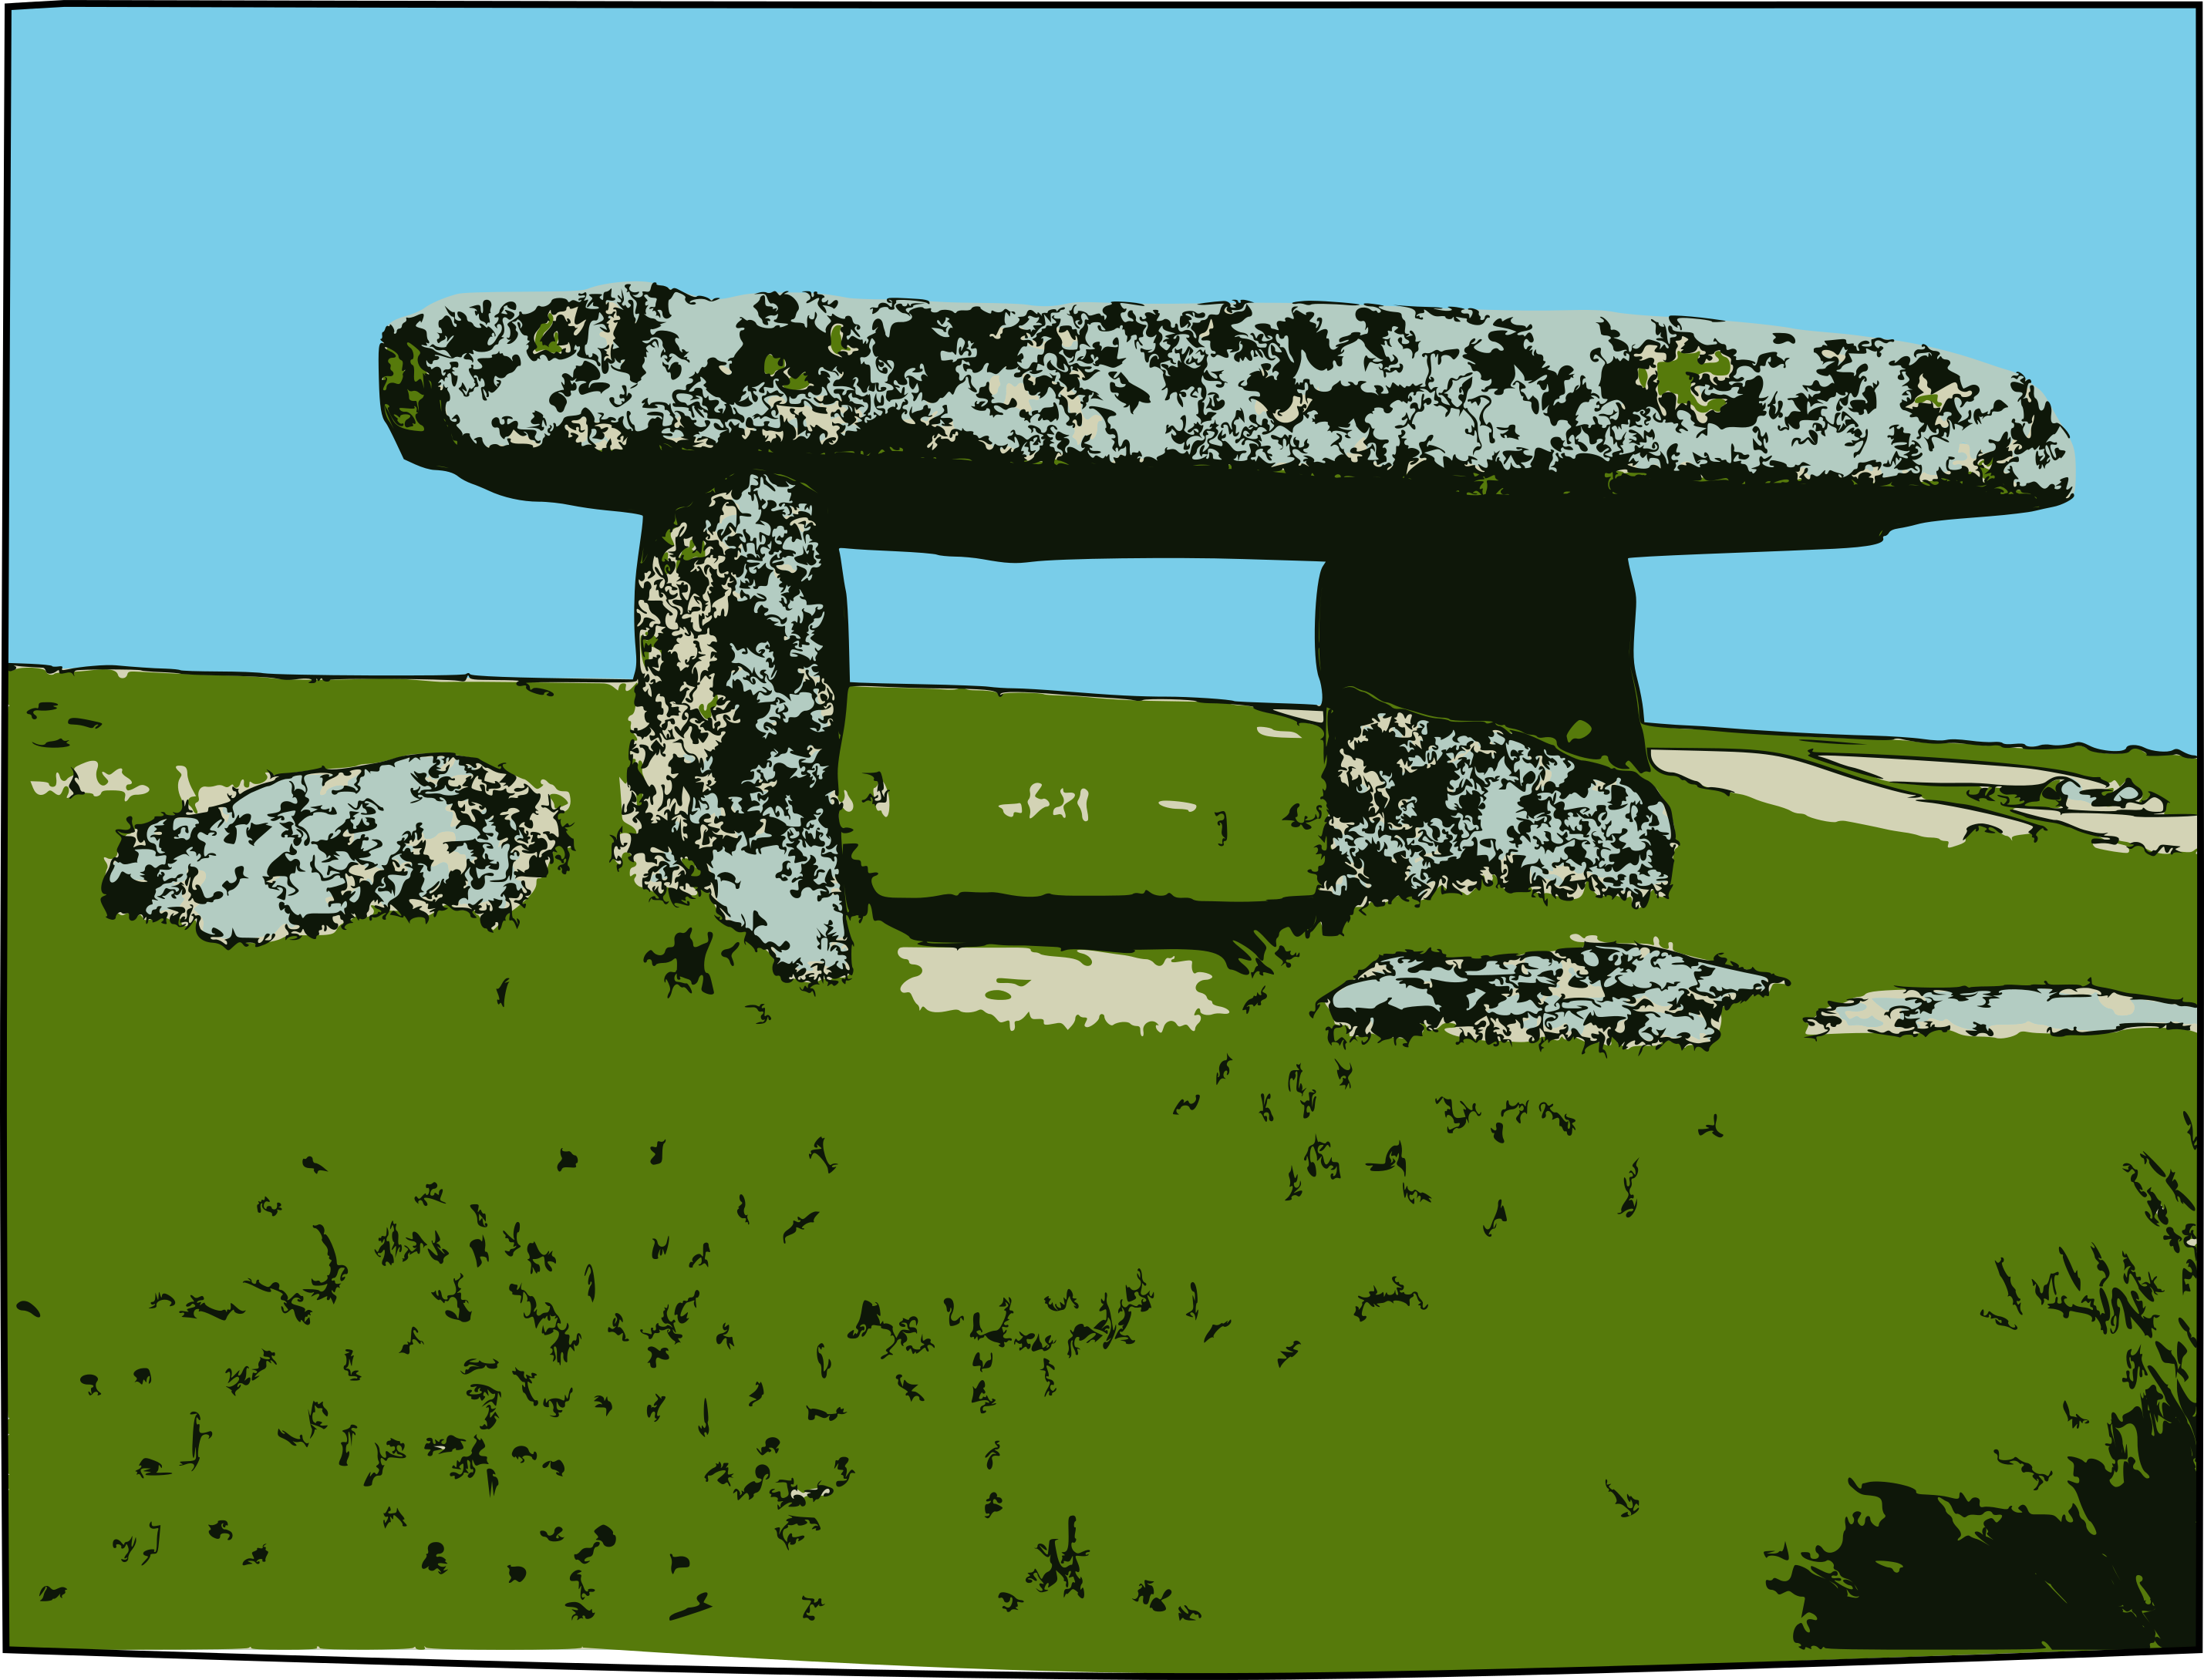
\includegraphics[width=5cm]{encyclopedia/dolmen}\caption[Dolmen*]{Dolmen near Pickham, Upwold*}\end{figure}
\paragraph{dragonbone} a clay-like soft material found near the roots of living trees, generally symbolised by a dragon's head. Used by magicksmiths to create \s{magickal item}s that affect bonds or the spirit.
\paragraph{drakes} the first marcher army, named after the first general, \s{Tom Drake}. Composed mostly of well-equipped \s{Mitwold}er yeomen.\begin{figure}\centering
\includegraphics[width=5cm]{encyclopedia/Drakes}\caption{Drakes emblem}\end{figure}
\paragraph{drake} large reptilian mundane creatures of a variety of shapes and sizes. They are usually predatory, and while the majority are man-sized or smaller there are a few uncommon breeds that are larger than a man. They are unkent in the cold north of the \s{Empire}.
\paragraph{druj} \s{barbarian} orcs well-versed in using herbal \s{poison}s and \s{potion}s, and creating auras of \s{fear}. On the battlefield the druj strive to project a terrifying image. They usually wear dark colours, suitable for hiding in bogs and swamps, often with hints of dark green and yellow.
\paragraph{dwile flinging} a \s{sport} from the area of \s{Greywater}. The game involves of two teams, each taking a turn to dance around the other while attempting to avoid an ale-soaked cloth, the dwile, flung by the non-dancing team. The jobbernoll (referee) awards points based on body parts hit by the dwile.
\paragraph{eastern guard} a fortification in \s{Birchland} in \s{Upwold}, originally built against \s{Dawn} and \s{vallorn}spawn from Miaren. The brooding towers and crenelated walls were built early in the history of the Marches in Birchland, on impetus of \s{Joshua Benson}'s tower at Pickham. The castle is a popular stopping place for merchants travelling through the central \s{Empire}, but still battle ready at all times, for one never kens when an attack may come from an unexpected direction. 
\paragraph{Empire} The republic founded by the \s{first Empress} on the idea of uniting humanity to bring ken of the way and of the true \s{virtue}s to every human (and, by current understanding, every other) soul. Composed of ten \s{nation}s tied together by one \s{throne} and \s{constitution}, and surrounded by heathen neighbours, the \s{Empire} is humanity's Civilization's only hope.
\paragraph{enchantment} a lasting \s{magick}al effect, often produced by a ritual. Every target can only be under one enchantment at a time, though for example an enchantment of a farm can also affect the yeoman who owns it.
\paragraph{enmity} (do not confuse with \s{amity}) means that an \s{eternal} is considered an enemy of the \s{Empire}, just as a \s{barbarian}. Aiding such an individual is a \s{crime}.
\paragraph{Ephisis} \s{autumn} \s{eternal} of ethical trade, good barter and fair exchange, preferably of actual material things (though this includes skill and time, including for mediation). She is kent for the security of her vaults and her dislike of curses. The eternal herself has never been seen, but trade with her is also possible through the \s{ritual} Ephisis' Scale [autumn \s{magnitude} 4]
\paragraph{eternal} Do your homework before messing with eternals! eternals are lord of a domain in a \s{magick}al realm. Eternals and can be considered enemies of the \s{Empire} (\s{barbarian}) when under enmity, or \s{foreigner}s when under amity. Unless under special circumstances, a citizen is far fore likely to encounter \s{herald}s of eternals than the eternals themselves.  They are alien, powerful and well documented creatures. For the eternals seen around Anvil, politeness is usually sufficient to navigate an encounter.
\paragraph{exemplar} An exemplar is an individual demonstrating exceptional \s{virtue}, and fulfilling at least 4 of the 8 signs of the \s{paragon}, but without doctrinal status. While exemplarhood may be the first step to transcendence, the exemplar is defined above all by their capacity to inspire. The synod has recognized two exemplars in the Marches, the legendary folk heroine \s{Bolstering Bill} of \s{Loyalty} and \s{Pickham}'s \s{Joshua Benson}, exemplar of \s{Vigilance}.
\paragraph{faith} the proven belief in the seven \s{virtue}s guiding the soul through the \s{labyrinth} unites the \s{Empire}.
\paragraph{farm} if a landskeeper does not ken how to run a farm, this is not the document to teach them. Farm rituals (blessing of the new spring; strong ox, golden sun; gathering the harvest) can be found in the \s{appendix}.
\paragraph{fear} fear is a false \s{virtue}. Some barbarians, such as the \s{druj}, can create auras of supernatural fear, which can only be countered through supernatural means, such as the banner of the bold (\s{magick}al items), hallows of items, individual anointment, or, for a short leap of bravery, heroic might or the mental disposition of \s{lineaged}. \proverb{Fear is worse than fighting.}
\paragraph{feast for the crows} a dangerous and very specific antidote for illegal \s{poison}s.
\paragraph{Feni} the Feni are primitive human \s{barbarian}s from wild places of the Marches. They paint their bodies in colour and, almost always with drowned greens and dirty yellows. They make extensive use of camouflage, which makes it easy for them to hide and to attack from ambush, which they do frequently. Inbred and backwards, Feni mostly keep to themselves, but at semi-regular intervals they lead raids into the Marches, as well as southern Wintermark and the northern brass coast. In these savage raids, they thieve everything they can get away with, and kill anyone who wants to prospect their hard-earned \s{Prosperity}. They dress primitively, using only leather and fur, and use spears and javelins, because they lack fundamental aspects of civilization, such as metal work. The \s{Applewood} levy is a community of \s{household}s that banded together after a particularly brutal raid by the Feni.
\paragraph{first Empress} The first Empress was Highborn, and the last to ride a legendary Highborn \s{horse}. After taking \s{liao}, she revealed that all human souls are re-incarnated on the same wheel, regardless of whether they were Highborn. She thus began steps to start the formation of the \s{Empire} such that Highborn reborn elsewhere would still come to know their heritage and the Way of \s{virtue}. From Highborn faith, the Empire came into being, changing the face of the world forever.
\paragraph{Fisher’s Rock} a black stone mound that emerges from the middle of the fens near \s{Greywater}, \s{Bregasland}. Atop it is a ruined tower ascribed to the \s{Sentinel}. It is said to be haunted, often showing strange lantern lights that lead people astray in the fens. The area around the rock sometimes yields treasures—old cups, coins, or sometimes more significant artefacts. As a result, many of the local clannish \s{merrow} spend their time as prospectors; although they are as likely to return bloated with poison and on the brink of death as they are to return with something of interest. 
\paragraph{foot-the -ball} a famous Marcher \s{sport}, in which two teams try to get a ball the size of a pig's bladder to a goal in the other team's field. Weapons other than sticks no longer than a forearm are not permitted in play, and any \s{injury}, traumatic or otherwise, is usually quickly remedied by the \s{physick}s on the field.
\paragraph{foreigner} broadly, foreigners are any person who is neither a citizen nor a barbarian. Foreigners are subject to the \s{law} and are accorded protection by it as if they were a citizen, but they do not otherwise enjoy the benefits of citizenship. However, \s{eternal}s, and the \s{herald}s of eternals, are not treated as foreigners (thereby receiving protection under the law) unless they are the subject of a declaration of \s{amity} made by the Imperial conclave. If a citizen forswears their oath to their egregore and thereby ceases to be a citizen they become a foreigner (and so still benefit from the protection of the law). Citizens and former citizens who fight against the \s{Empire} will be given \s{trial}s for their crimes, rather than be treated as barbarians, if feasible. \begin{figure*}\centering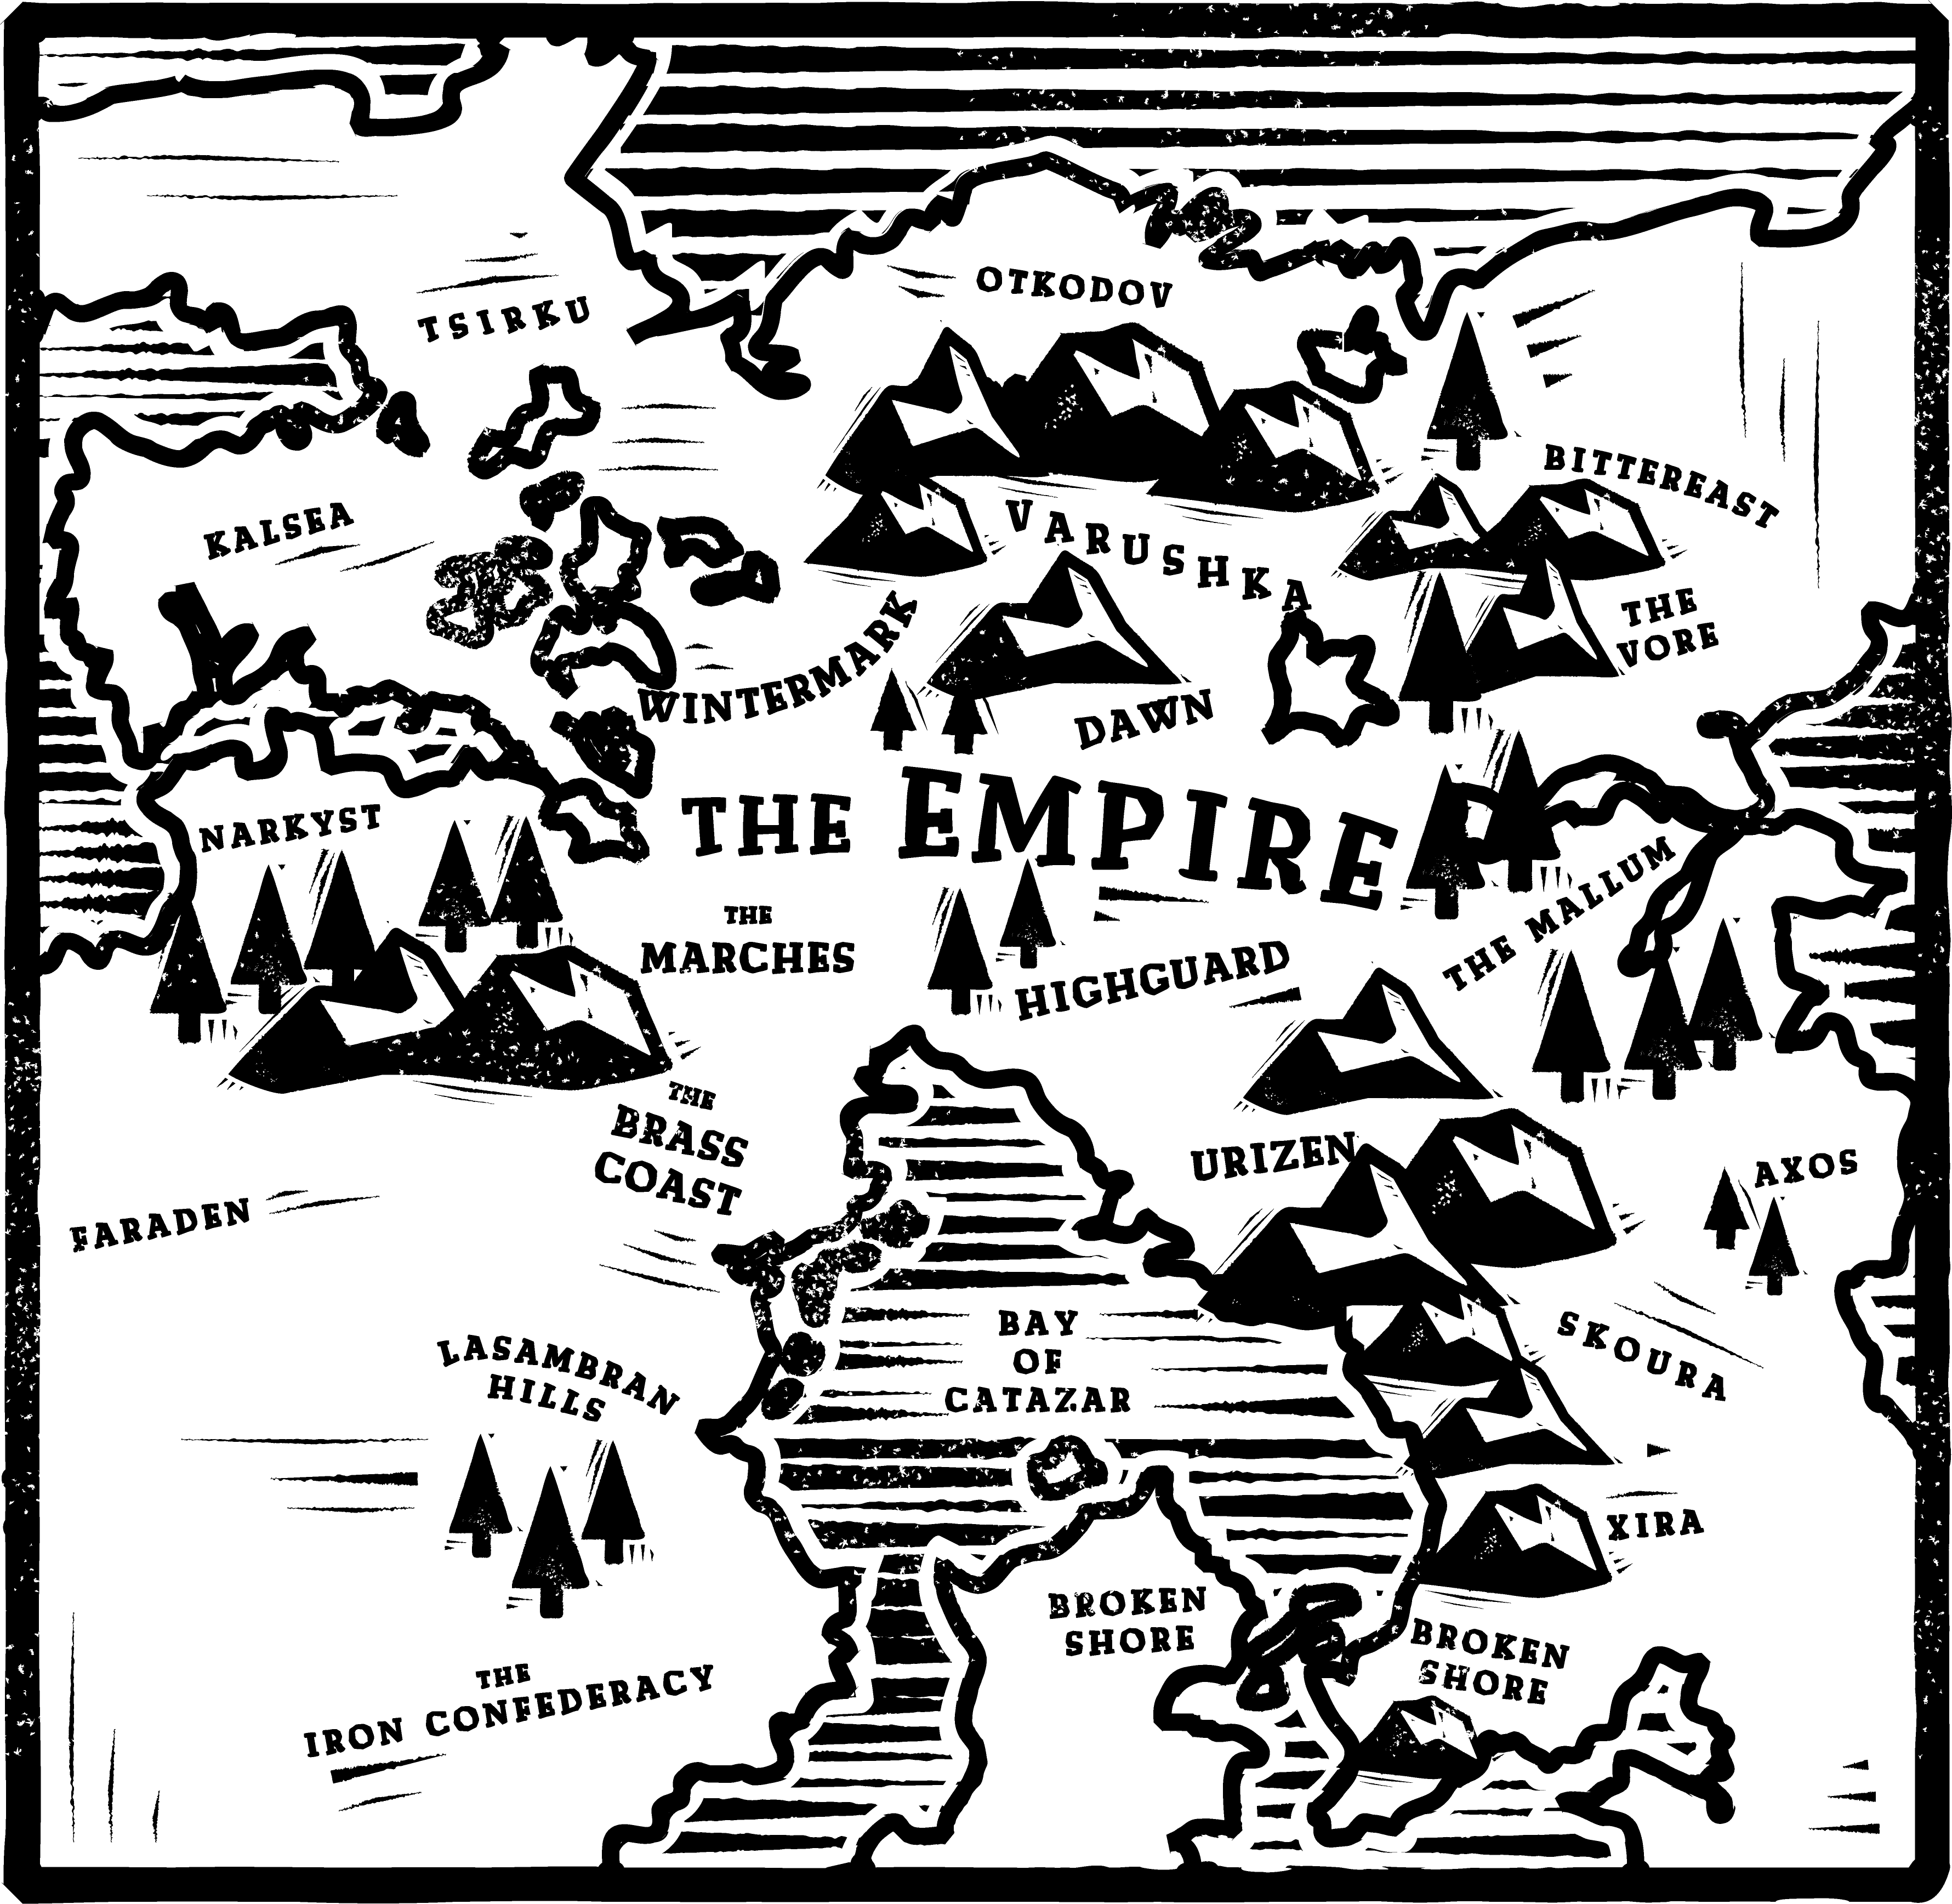
\includegraphics[width=0.9\textwidth]{encyclopedia/worldmap}\caption{the Empire and its neighbours}\end{figure*}
\paragraph{Forte Fidelis} old asavean for Faithful to the Luck. A fortification around \s{Hay} in \s{Mitwold}.
\paragraph{freeborn} an inhabitant of the \s{brass coast}.
\paragraph{Freemoor} a region in the northern \s{Mournwold}, held by the \s{jotun}.
\paragraph{friar} a pilgrim who has made following the way and teaching the \s{virtue}s his purpose in life. Often addressed as “brother” or “sister”.
\paragraph{Golden Downs} the region around \s{Hay} in \s{Mitwold}, containing the garrison \s{Forte Fidelis}.
\paragraph{Good Walder} \s{paragon} of \s{Prosperity}. Probably an early \s{landskeeper}. Usually depicted with a club and a straw mask.\begin{figure} \centering 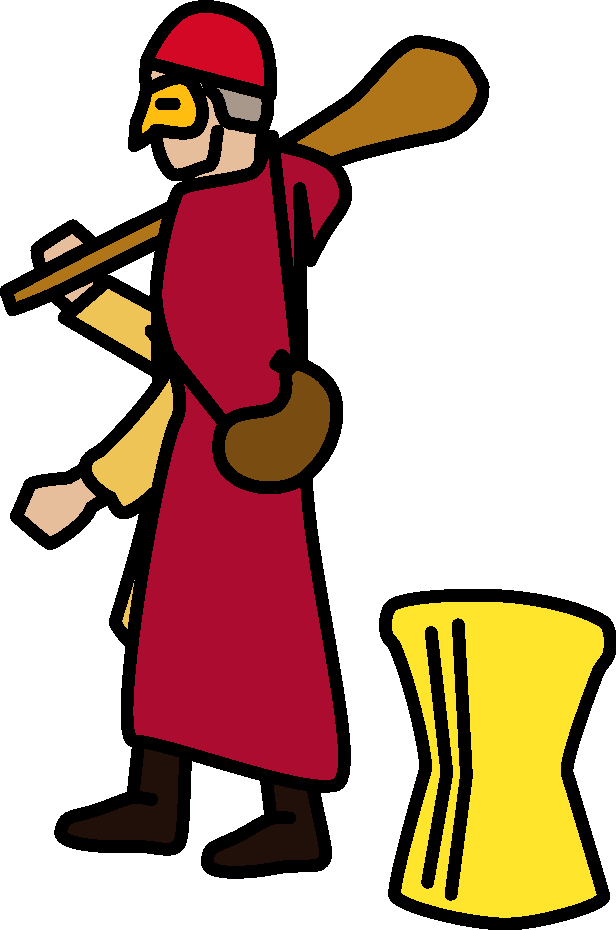
\includegraphics[width=5cm]{encyclopedia/Walder} \caption{Good Walder*}\end{figure}
\paragraph{grand market} a market in \s{Meade} which takes place on the third weekend of each month and attracts traders from across the Marches and even occasionally from Wintermark to the north. 
\paragraph{granite} \see{white granite}
\paragraph{Gravenmarch} the region around \s{Graven} in \s{Bregasland}.
\paragraph{Graven} \s{market town} in \s{Bregasland}. Graven grew rich from Graven Rock, its high fields and mineral wealth. In happier times the \s{navarr} came here often, with news and trade-goods from far afield. Many's the inhabitant here who started life far, far away, brought here by a navarr Guide. Nowadays, it’s the base of supply for the castles and forts that defend Bregasland against the \s{jotun} in the \s{Mournwold} and the forests of Liathaven.
\paragraph{green iron} a gray metal, generally symbolised by a sword. Used by magicksmiths to create dyes or lightwight \s{magickal item}s that offer protection.
\paragraph{Green March} a region in the \s{Mournwold}, held by the \s{jotun}.
\paragraph{Greensward} the region around \s{Overton} in the \s{Mournwold}, the only region in the Mourn held by the \s{Empire}. Can also refer to the Overton Monastery.
\paragraph{grendel} orcs who hail from lands to the south and east of the \s{Bay of Catazar}. A nation of sea-faring orcs with a love for wealth and power, they were once nothing but \s{pirate}s and reavers. Over time their society has advanced to the point where they are as likely to trade as to steal what they want. Despite the luxurious lifestyle of their leaders, the \keyword{Salt Lords}, the Grendel are brutal, uncompromising bullies who use violence and threats of violence to get what they want. On the field of \s{battle}, the grendel field mercenary orc tribes, as well as their own elite moridun.
\paragraph{Grey Fens} The region around Greywater in Bregasland.
\paragraph{Greywater} village in \s{Bregasland}, the furthest west any wise Marcher will go. The locals make their living primarily from eel-fishing, but since this isn’t a trade that leads to many exports, some of the more daring amongst them will scour the surrounding marsh for unusual plants and flowers. These are dried, and sold through the markets at Meade. The local grey water is not the best water to drink, so there's a thriving market in pure water.
\bigparagraph{group} Citizens of the \s{Empire} are organized into groups on various levels. \localpar \keyword{National} In the Marches families, groups of individuals sharing common descent, can often recognized by sharing a surname. A \s{household}, \s{market town} or \s{monastery} is formed by individuals from the same location, bound in \s{loyalty} to a \s{steward}, \s{abbot} or \s{alderman} chosen from among them. They generally have members from multiple families, even though often one family is dominant—in particular in the case of households, which are often named after that family. \localpar \keyword{Bands} For the purpose of metaphysical benefits, people of the \s{Marches} or other nations often band together by magick under one common oath, forming \s{banner}s, \s{coven}s and \s{sect}s. The metaphysics of the world require that each Imperial citizen be a member of at most one banner, at most one coven and at most one sect, and because they draw upon the magick of the \s{egregore} spirit, all members of such a band must be members of the same \s{nation}. \localpar \keyword{International} Beyond the Marches, Imperial citizens form sodalities representing a serious and enduring commitment to an Imperial cause across the nations, such as the \s{Imperial School of Medicine} providing, among other things, the \s{Anvil} hospital; the Purple Sail, encouraging trade with foreign nations; or the Three Refrains, which was formed by bards to uphold the musical traditions of the nations irrespective of political interests. The \s{conclave order}s are sodalities of a particular nature in that they are metaphysically bound by the \s{ritual} arcane mark, ensuring that every magickian can be a member of only one order, and in that their grand masters have special powers in conclave. \localpar \keyword{Constitutional} Lastly, the constitutional bodies of \s{synod}, \s{senate}, \s{conclave}, \s{bourse} and \s{military council} form groups of a special nature, instituted to find, distill and execute the will of the Empire as a whole.
\bigparagraphendtwiddle
\paragraph{hallow} a ceremony that gives a magickal item an aura of \s{virtue}, affecting everyone bound to the item.
\paragraph{hat} a fundamental piece of Marcher garment \proverb{I'll just go and put my hat on.}
\paragraph{Hay} a small rural town set amongst rolling field in southern \s{Mitwold}, near the border to the \s{jotun}-occupied \s{Mournwold}. “The golden fields of Hay” appear in many a Marcher song.
\paragraph{headpant} also kent as “coif”, a piece of garment worn on the head. Worn under a hat or helmet, it can prevent chafing.
\paragraph{hearth magick} is a low-key everyday type of magick that keeps us being safe and prosperous. It is also important for keeping the \s{Jack-in-chains} bound. Important elements of Marcher hearth magick are the appropriate burial of Marchers in Marcher soil after \s{death} (cf. \s{holberg}), and many elements of tradition, such as \s{poppet}s and seasonal festivals, grant the Marchers persistent Prosperity through hearth magick.\proverb{The answer lies in the soil.}
\paragraph{hearth tithe} an ancient tradition in the Marches and \s{Wintermark}, where farmers diversify their farms to grow \s{herb}s in addition to food to support their communities in times of war. The practice largely fell out of practice during the Second Interregnum. It was common for \s{monk}s to encourage the observation of the Hearth Tithe. A \s{monastery} would often receive donations of herbs from the surrounding farms to be used in support of the wider community. The practice has not been widely observed for over a century, but was reintroduced in the year 379.
\paragraph{Heath} a region in \s{Upwold}, containing the \s{Sutton quarries} and bordering the \s{Mournwold}.
\paragraph{hedge wizard} a \s{magick} user whose main \s{Loyalty} is a single \s{household}, not the whole of the Marches.
\paragraph{hedges} a line of shrubs and important marker of the boundaries (\s{beater}) of fields and communities. As of new, it has become a tradition to bury dead \s{briar}s in the brambles of hedges. \proverb{A hedge between keeps a friendship green.}
\paragraph{Hepton bridge} Some of the worst fighting of the short-lived \s{Marcher civil war} took place in western Upwold; one of the few pitched battles between the supporters of the \s{first Empress} and those households who opposed the formation of the \s{Empire} took place here at Hepton Bridge. Perhaps the bloodiest conflict of the civil war, the scrubby heathland of the battlefield is largely given a wide berth except by occasional pilgrims of Loyalty who come here to muse on the spiritual significance of the ancient conflict that set cousins against one another. 
\paragraph{herald} More human, both physically and socially, servitors of the \s{eternal}s. These can be recognised by their alien forms (Heralds usually show strong signs of lineage or similar exotic features such as beaks, horns, feathers etc.) and their detection under magick.  Nearly every herald encountered within the \s{Empire} will belong to an eternal under \s{amity} and be considered a \s{foreigner}, because protective magick makes it hard for other heralds to enter this realm. They will generally be honest about their master. They will exhibit character traits consistent with their master. They can be powerful creatures and unless you ken better should be treated with a similar respect to a stranger in the inn. You ken, the one that you're not sure whether they will stab you in the alley, bring news from a far away place or offer trades that greatly benefit you.
\paragraph{herb} in addition to herbs useful in cookery and brewing, Imperial herb gardens grow five herbs with important applications in \s{medicine}. \begin{table} \begin{tabular}{p{0.6\textwidth}} blue mazzarine to save a limb\\ grey bladeroot stems a weakness dim\\ red roseweald venom’s power breaks\\ true vervain body's healing wakes\\ though marrowort takes soldiers' pain\\ at battle's end they'll fall again\\ \end{tabular}\caption{medical herbs}\end{table}
\paragraph{herding cats} a fine skill for any landskeeper.
\paragraph{heresy} the religious \s{crime} of willfully rejecting, or perverting, the orthodox doctrines of the faith as laid down by the Imperial synod, or actively teaching and promoting false doctrines.
\paragraph{high Courage} a monument in the \s{Green March} near the border with \s{Bregasland}. Looking down across the moors towards Liathaven, it is a large statue of a stag with broken antlers, ascribed to the people of Terunael (who later became the \s{navarr}). On a stone block at the base of the statue letters simply read “High Courage” but it is clear that they are more recent than the statue itself. \begin{figure}\centering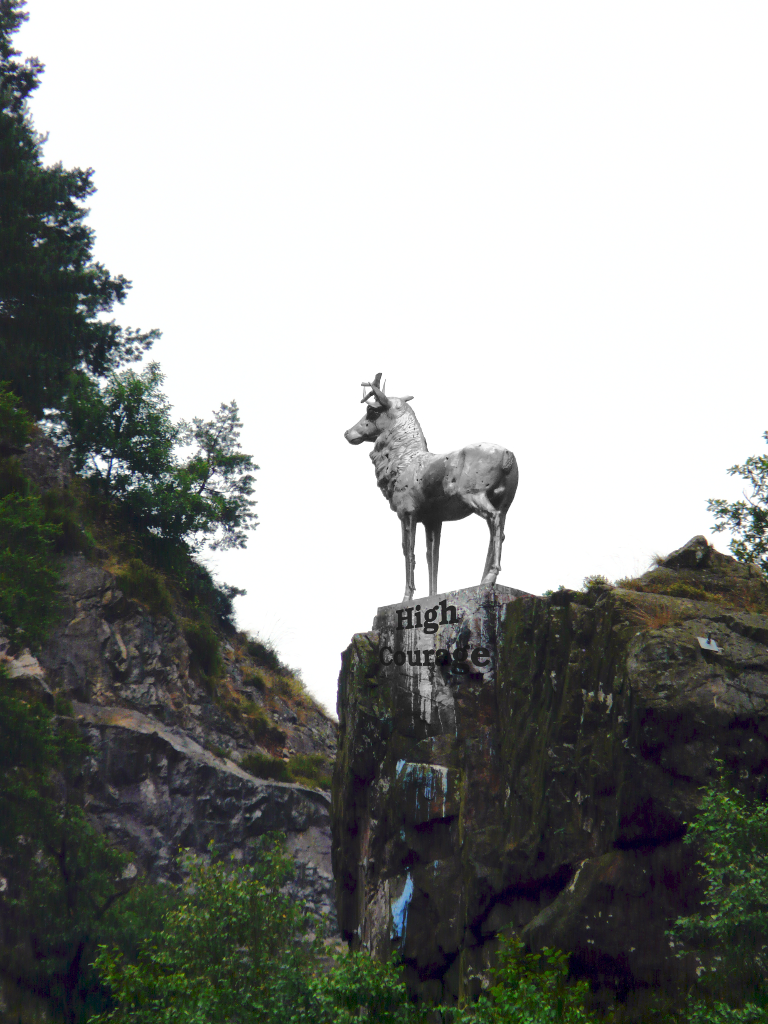
\includegraphics[width=5cm]{encyclopedia/highcourage}\caption{high Courage*}\end{figure}\footnotetext{by Frank C. Müller}
\paragraph{highguard} the \s{nation} that created the Imperial \s{faith}.
\paragraph{holberg} the easternmost city of the \s{League}, notable for containing small enclave of Marcher soil in the League, where Marchers were put to rest. The establishment was necessary because the bodies had been animated through a \s{winter} \s{ritual} to fight in the liberation of the city from the \s{druj}, which interfered with Marcher \s{hearth magick} concerning \s{death} and awoke \s{Jack-in-chains}.
\paragraph{horse} an extinct four-legged draft animal and mount, symbol of \s{Loyalty} and the whole \s{Empire}. The fleet settling highguard carried with them a great herd of horses, but mismanagement and greed led to their exctinction about the time of the foundation of the \s{Empire}. The \s{first Empress} was the last owner of a proud war horse, and so the horse has become a symbol of the \s{Empire}.\begin{figure}\centering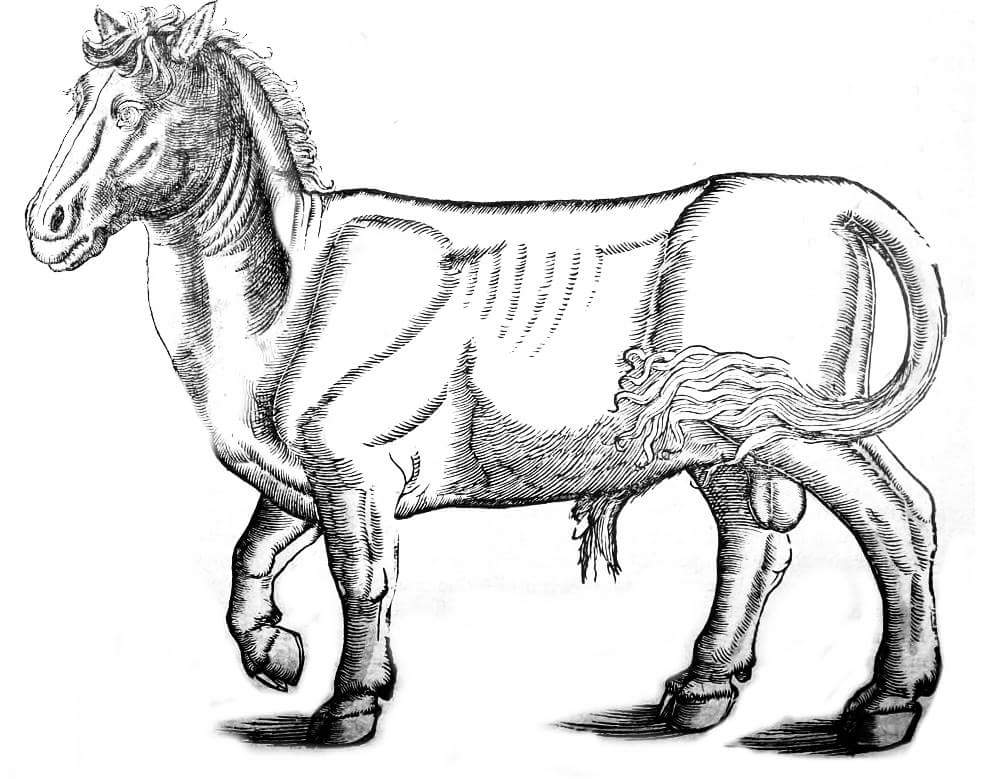
\includegraphics[width=5cm]{encyclopedia/Horse}\caption{horse (reconstruction)*}\end{figure}
\paragraph{household} a group of \s{yeomen} and supporting people, such as \s{friar}s, \s{magicksmith}s and \s{hedge wizard}s, from the same area who have selected one of theirs to act as their \s{steward}. They are bound by their \s{Loyalty} to each other because they have common economic, political or military interests.
\paragraph{hunger} is a sign of lack of \s{Prosperity}. Unfortunate Marchers are welcome to help themselves to the fruits of the grave-orchards, and many places such as monasteries give support to increase the Prosperity of downtrodden Marcher folk. In Anvil, hunger can be alleviated by dining at tyke’s.\proverb{He who lives on hope, dies of hunger.}
\paragraph{husk} an animated corpse, eg. created by \s{winter} magick or \s{vallorn}. May need \s{burial} (cf. \s{holberg}).
\paragraph{idolatry}the religious \s{crime} of subsuming human will and destiny to any inhuman entity or force. This includes the worship, veneration or exaltation of any such being or power.
\paragraph{ilium} star metal, a valuable material with strong magickal properties. One of the four strategical Imperial resources, distributed by the bourse. Ilium can make magick effects permanent.
\paragraph{Imperial lore} the collected body of formulaic \s{ritual}s generally kent throughout the \s{Empire}. Every magickian has enough passing familiarity with the rituals associated with their \s{lore} to contribute to one of these, even when they have not \s{mastered} it.
\paragraph{Imperial roseweald} one of the apothecary \s{herb}s.
\paragraph{Imperial school of medicine} a \s{sodality} dedicated to the protection and promotion of the healing arts. Founded upon Marcher initiative, the sodality also runs the Anvil field hospital. Anyone with an eager interest in the medical arts of a chirurgeon, physick or apothecary will find much more intensive discussion of those matters in their wise library than in this loyal compendium.
\paragraph{injury} damage to the body, mitigated by \s{medicine}.
\paragraph{inquisition} a formal process through which the \s{synod} assesses how virtuous or unvirtuous an individual or group is. An individual or group may only be subjected to inquisition once per summit. Whoever faces inquisition must come to a designated location at a set time. The duration of the inquisition is one hour, which can be extended by a \s{magistrate}. Refusing to participate in an inquisition can be ground for escalation to condemnation, the lack of co-operation will be taken into consideration by the magistrate and might be considered a \s{crime} against the processes of state. An inquisiting priest may call for a condemnation, which does not count as raising another synod judgement but is an extension of the inquisition, and will lead to a \s{trial} according to the \s{law}.
\paragraph{insight} a priestly ceremony that allows a \s{friar} to discern a mark on someone's soul.
\paragraph{iridescent gloaming} the wax from iridescent butterfly cocoons, generally symbolised by a butterfly. Used as colouring agent by magicksmiths who create \s{magickal item}s to enhance magick.
\paragraph{iron raptors} a \s{mercenary} bands, undertaking private commissions to remove bandits and monsters for coin and glory. The iron raptors can sometimes be found in \s{Anvil} looking for desperate yeomen willing to go on their \s{skirmish}es for coin and bounty.
\paragraph{ISoM} \see{Imperial school of medicine}
\paragraph{Jack-in-chains} the dark mirror of the Marcher egregore \s{Jack-in-the-green}. Same name as an evil giant from a children's story, also kent as Jack-of-Irons or Bloody Jack. Legend has it that Jack-in-chains was tricked into falling down a well and is still buried near \s{Wayford}.
\paragraph{Jack-in-the-green} the Marcher egregore. As every \s{nation} of the \s{Empire}, all Marchers are bound to an egregore. Some generations until 379, the egregore's spirit inhabited Robert Ramsbruck, a \s{beater}. After he fell in battle fighting a \s{drake}, Jack found a new host in the herbalist Fern. The power of Marcher \s{hearth magick} keeps his dark counterpart, the \s{Jack-in-chains}, bound deep in his core. If Jack-in-chains gets loose, he needs to be bound again by Marchers following their traditions, and innocent \s{soul}s binding him in place, just like in the old legends we ken of the Jack-in-chains. The figures of Jack-in-the-green and Jack-in-chains may actually be older than the formation of the \s{Empire}, for they have been part of legends even when the \s{Empire} was founded.
\paragraph{Joshua Benson} \s{exemplar} of \s{Vigilance}, recognized by the \s{synod} in 378. Known as “the major”. He is usually depicted on top of a tower with a shield, holding watch.\begin{figure} \centering 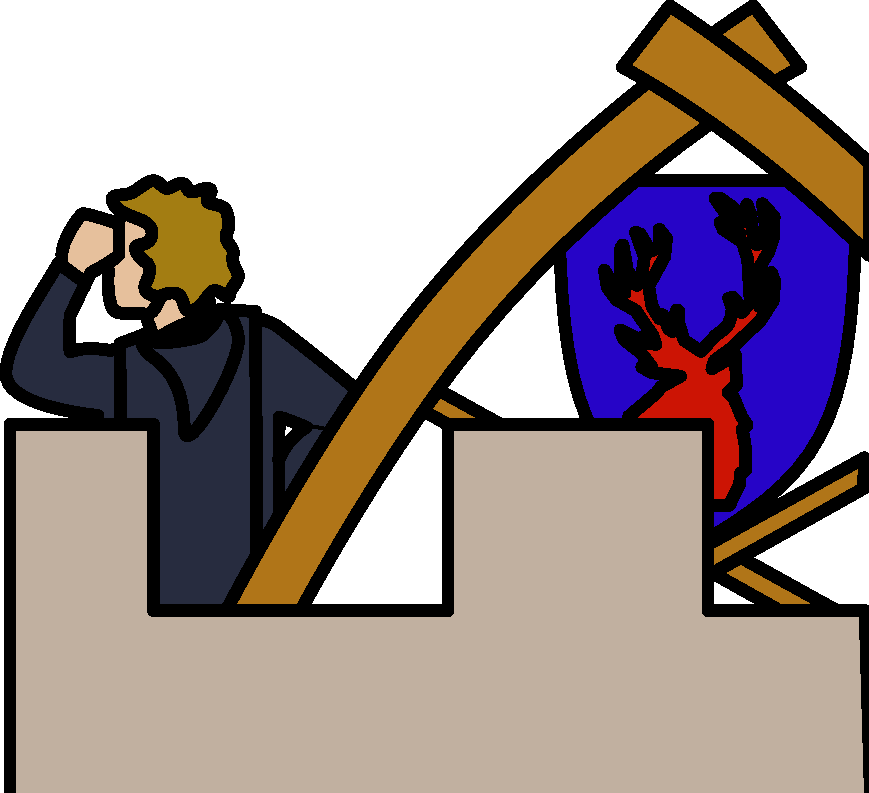
\includegraphics[width=5cm]{encyclopedia/Major} \caption{Joshua Benson*}\end{figure}
\paragraph{jotun} the tribe of \s{barbarian} orcs that have captured the \s{Mournwold} in 347. They are a warlike tribe that values strength-in-arms and fighting-spirit as their highest \s{virtue}s; they love one-on-one fights, challenged by the orc pointing at an opponent with their weapon and then raising their head up to show their necks to their opponent. Making a slashing or ripping gesture with their hand as they bring their head down with a snarl. This signal shows that they consider the person they are looking at as worthy of honourable combat. The target may return the challenge, and engage the jotun in single combat that ends until one warrior cannot continue. jotun will usually accept a surrender unless they have reason to believe they are being tricked in some manner, and often allow injured opponents to retreat. They have also been kent to allow opponents who have fought bravely to gather their dead or injured. Warriors of the jotun see little honour in killing the weak or the unarmed, and prefer to take them as thralls. Thralls are treated reasonably well by the jotun; as long as they show proper respect to their overlords, they are usually left to their own devices. Many modern jotun thralls are the descendants of humans taken in battle, and consider the \s{Empire} their enemy. The jotun value Courage, strength and martial prowess above other attributes. Their love of battle and emphasis on personal glory and honour, as well as their war-like traditions, means that many jotun warriors are a match one-on-one for their Imperial counterparts. They do not throw their lives away, nor use their subject tribes as disposable troops, but they are invariably looking for a way to increase their honour, with an eye towards becoming ancestors when they die. The only true dishonour most jotun recognise is showing fear in the face of the enemy, or striking a worthy opponent down by treacherous means. jotun favour axes and hammers, both two-handed and coupled with a round shield. They tend to shy away from bows, and seem to have no appreciation for the crossbow as a weapon of war—when it comes to ranged combat they prefer thrown axes or javelins. The colour red appears to have totemic significance for the jotun, and figures on most of their banners. \proverb{Better an honest enemy than a false friend.}
\paragraph{judgement} a decision of the \s{synod}
\paragraph{Kallavesi} one of the three traditions of \s{Wintermark}
\paragraph{King's Stoke} \s{market town} in \s{Upwold}, with a tower that existed before the \s{march}, possibly built by the \s{Sentinel}.
\paragraph{labyrinth}the twisting realm of pure spirit that is integral to the cycle of reincarnation, a core doctrine of the \s{faith}. The name is something of a metaphor for no mortal has been there to witness it, but the journey from death to rebirth is neither simple nor instantaneous. Some spirits are said to wander between lives generations before being reborn, and some are lost forever. The way of \s{virtue} teaches that living a virtuous life holds the key to successfully traversing the labyrinth of ages swiftly, safely and with the purity of spirit that strengthens ties to past lives.\begin{figure} \centering 
\includegraphics[width=5cm]{encyclopedia/Labyrinth} \caption{the  labyrinth symbol}\end{figure}
\paragraph{landskeeper} anyone who uses \s{magick} to support the Marches as a whole and Marcher folklore in particular. Landskeepers can use a variety of methods, from \s{hearth magick} to \s{ritual}s, to do this. Some landskeepers lack education in specific magickal abilities at all, and use traditional rites and offer good advice and aid to the Marcher folk. Many landskeepers avoid the conflicting loyalties arising from also being part of a \s{household} and look down on \s{hedge wizard}s who put their Loyalty to a \s{steward} above Loyalty to the Marches.
\paragraph{landskeeper's oath} The oaths that landskeepers swear are often carved into a a tree, to bind them to the land. By extension, a magick staff crafted from such a tree, which can allow a battle magickian landskeeper to bind enemies in place, is called a landskeeper's oath. \proverb{As easy to escape as a landskeeper’s oath.}
\paragraph{Lashonar} \s{night} \s{eternal} of speech and active communication facilitating change, and travel. Heralds of Lashonar often have a bird-like appearance, and many have a reputation for being petty thieves, and tend to view visits to the mortal realm as an amusing holiday rather than a serious duty. Lashonar delights in speech, be it singing, drama, debates, or rumour; and the solving of mysteries. It loves to hear secrets, but often finds itself at odds with the \s{Whisper-Gallery}. While those hoard secrets, Lashonar effectively destroys them by sharing them. 
\paragraph{law} Marcher business is Marcher business, and should be conducted as such. Tradition has means to settle \s{boundary dispute}s, \s{sorcerer}s, and so on. But when individuals from elsewhere are involved in an affair, the Imperial code of law applies. This is often the case for events related to a summit in Anvil. Under Imperial law, \s{foreigner}s have the same protection as \s{citizen}s, though not the same rights. \s{barbarian}s do not have those rights, quite the opposite. Imperial law regulates crimes against people, crimes of position, crimes against the state, civil claims and religious crimes. The decision on guilt and punishment is made by a magistrate in a \s{trial}. The corresponding tables list all criminal acts; It is possible for willing participants to give consent so that what would otherwise be crimes being committed against them are not. Attempting, ading or abetting of a crime is equivalent to committing the crime under the law. \begin{table*}\begin{tabular}{p{0.15\textwidth}p{0.75\textwidth}} Murder& action against a person with intent to kill them.\\ Manslaughter& against a person which results in someone’s death.\\ Assault& striking a citizen. (Lack of lasting injuries can make fights legal.)\\ Mayhem& maiming or mutilating a citizen.\\ Poisoning& applying a poisonous substance or effect to a citizen which causes them harm.\\ Imprisonment& Unlawfully detaining a citizen against their will. Suspects must be directly supervised during any period of lawful custody.\\ Malsanguino& Willfully preventing someone from receiving medical attention with the intention of causing them harm.\\ Slavery& holding the power of life and liberty over any person, including \s{barbarian}s. \end{tabular}\caption{crimes against the person}\end{table*}\begin{table*}\begin{tabular}{p{0.2\textwidth}p{0.7\textwidth}}Theft& Dishonestly appropriating property belonging to another with the intention of permanently depriving the other of it.\\ Counterfeiting& falsifying, creating or amending of an Imperial document or legal tender.\\ Criminal Damage& destroying or damaging any property either belonging to another citizen or to the \s{Empire}. \\ Breach of interdict & Owning forbidden items and substances. This includes drake's eggs, vallorn seeds, the Maggothe s Talon wand, and the poisons gutwrench, moon's poison, hunger of the wolf, black gate and crimson gate. (for items interdicted by the conclave, the crime is against the processes of the state.)\\ Vallorn cultivation& Planting or tending vallorn is very likely to be interpreted to be vallorn cultivation, harvesting magickal ingredients from a naturally occurring vallorn pod may or may not be.\\ Trade of True Liao to foreigners& It is illegal to trade True Liao to anyone who is not a citizen.\\\multicolumn{2}{l}{\textit{Cases of negligence \&c. can be brought before forward in civil trials.}} \end{tabular}\caption{crimes against the property}\end{table*}\begin{table*}\begin{tabular}{p{0.22\textwidth}p{0.68\textwidth}}Treason& Aiding barbarians, eternals, or foreign powers to act against the interests of the \s{Empire}. Committing an assault against the emperor or empress. \textit{Only citizens and former citizens of the \s{Empire} may be charged with treason.}\\ Impersonation of an Imperial Official& Falsely and dishonestly claiming to be a senator, civil servant, member of the militia \&c., with intent to deceive.\\ Dereliction of Duty& Volunteering for an Imperial duty and then failing to carry it out through neglect or cowardice. \textit{abuse of an Imperial position is within the remit of the Synod.}\\ Vyig Membership & Membership in the criminal organisation, or possession of Vyig tattoos. \end{tabular}\caption{crimes of position}\end{table*}\begin{table*}\begin{tabular}{p{0.25\textwidth}p{0.65\textwidth}}Contempt of Court& any behaviour which impedes the proper operation of the legal process, such as disrupting a trial, or failing to attend court.\\ Perverting the Course of Justice& any behaviour calculated to unduly affect the course of the judicial process, such as bearing false witness, making false allegations, concealing offences or assisting others to evade arrest, interference with witnesses or evidence and evading, withholding or perverting a lawful punishment.\\ Subverting agencies of the state& any behaviour which contravenes or subverts the constitutionally protected procedures or powers of an agency of the state. \\ Resisting Arrest& Any course of action with the intent to oppose a lawful arrest.\\ Contravening a Declaration of Sorcery& as a declared sorcerer, owning crystal mana, performing rituals or interacting with Heralds and Eternals.\\ Improper placement of an aura on the senate building& The placing of an aura on the senate building without prior explicit permission from the Senate.\end{tabular}\caption{crimes against the processes of the state}\end{table*} \begin{table*}\begin{tabular}{p{0.15\textwidth}p{0.73\textwidth}}Idolatry& Subsuming human will and destiny to any inhuman entity or force. This includes the worship, veneration or exaltation of any such being or power.\\ Blasphemy&The denigration of the Paragons and the Paths of Virtue. This includes promoting False Virtues and the teachings, or example, of False Exemplars or False Paragons.\\ Heresy& The willful rejection, or perversion of, the Orthodox Doctrines of the Faith as laid down by the Imperial Synod, or actively teaching and promoting False Doctrines.\\ Abuse of Powers& The misuse, or abuse, of the powers of a priest. This includes the powers of the Synod, as well as liao ceremonies.\\ Desecration& The removal of spontaneously created auras such as legacies of ascendance to \s{paragon}hood. This includes such auras arising on areas, objects and people. \\ \multicolumn{2}{l}{\textit{Religious Crimes are tried by a magistrate but are raised by the Imperial Synod.}}\end{tabular}\caption{religious crimes}\end{table*}
\paragraph{League} a \s{nation} of city-dwellers, attempting to have \s{Meade} declared a free city and rolled into their nation. \s{holberg} is the easternmost city of the League.
\paragraph{liao} a refinement of vinum, used in a priestly \s{ceremony}. The very rare, pure liao allows citizens to experience visions of past lives.
\paragraph{lineaged} lineage means that a person is touched by one of the \s{magick}al realms and can occur in many ways. The table gives an overview of the types of lineage and their associated realms. Parents with lineage often give birth to children with their lineage, while the offspring of a human and a \s{herald} is always lineaged. It is also happens that fully human parents give birth to a lineaged child. Lineage can also occur for other reasons, for instance a child born in a primal forest under the influence of the realm of spring might become a \s{briar} in later life while a child born during a great famine when winter holds sway might be born a draughir. At certain times, the flow of magick due to constellation on the sky can influence the occurrence of lineaged, either naturally or by making transformative magick easier. Many Marcher households are kent to not include any lineaged, despite appearance to the contrary – denying the merrow lineage of a household member by stating that they would be a mere human who is just feeling a bit blue –, or insist, for example, that their good cambions are spirited and energetic, whereas a cambion stranger would be seen as particularly conniving.\begin{table*}\begin{tabular}{lll} name& realm& trappings\\ \hline \s{briar}& spring& bark; volatile, impulsive \& restless behaviour\\ changeling& summer& pointy ears, antlers; bold \& self-confident attitude\\ cambion& autumn& curved horns; opinionated \& driven dominance\\ draughir& winter& pale skin, hollow eyes; cold \& hungry desire\\ \s{merrow}& day& gills, blue mottled skin; calm \& focused distance\\ naga& night& scales; relaxed \& passionate indulgence\end{tabular}\caption{lineages}\end{table*}
\paragraph{lore} a measure of how well versed a ritualist is in a particular \s{realm}'s \s{magick}. This is the limit of how much \s{crystal mana} they may channel into a \s{ritual}. \textit{contrast} the body of \s{Imperial lore}
\paragraph{Loyalty} a \s{virtue} \proverb{A chain is only as strong as its weakest link.}
\paragraph{magickal item} craftsmen can use the rare materials orichalchum (o), iridescent gloaming (ig), beggar’s lye (b) ambergelt (a), tempest jade (j) green iron (g), dragonbone (d), weltsilver (w) to create magickal items. Such items retain their special function for 4 seasons, after which they have to be re-charged, essentially creating the magick again from scratch. It does mostly take a \s{magicksmith} a full month to create an item; for such items as are empowered by skillful application of the artisan’s craftsmanship alone, and not through the magickal properties of their materials, it takes a magicksmith 2 full months. Personal magickal items can be armour, weapons or talismans (including shields). A magickian needs to create a bond between the bearer and the item, and every citizen can only have one bond of each of the three types. magick jacks or mithril mail can still be worn under good steel. In addition, a group can have a magickal banner, covenstone or reliquary, and such item can aid every member of the group. The late Pete Keeper of \s{King's Stoke} has analysed and composed a selection of inexpensive, useful equipment for the soldiers of a Marcher household, which is reproduced here for convenience. \begin{table*}\centering\begin{tabular}{p{0.9\textwidth}}{\parindent=-1em bolstering bill: a dying comrade may be saved once a day. 6 g, 7 w.}\\\parindent=-1em  butcher’s bill: cleave a foe in twain or bowl them down once a day. 8 o, 2 ig\\\parindent=-1em  warden’s bardiche (bill): another surge of heroic might. 10g 3 a\\\parindent=-1em  reaving mattock (great weapon): shatter an armament once a day. 7j\\\parindent=-1em  oathkeeper’s bow: another surge of heroic might. 8 g 5 a\\\parindent=-1em  biting blade: this side-sword will cleave a foe mightily once a day. 7 o.\\\parindent=-1em  stoutheart gambeson (light jack): an extra degree of fortitude, slowing the wearer’s bleeding. 2 months of a magicksmith’s time.\\\parindent=-1em  winter’s breath (light jack): cure three of your wounds once per day. 5w 5a.\\\parindent=-1em  soldier’s harness (light jack): the yeoman soldier may suffer another blow before she falls. 8a\\\parindent=-1em  mediator’s mail (medium weight): cure three of your wounds with heroic might. 2 months of a magicksmith’s time.\\\parindent=-1em  mithril shirt (medium weight): the yeoman soldier may suffer another blow before she falls. 2o 4a.\\\parindent=-1em  warrior’s plate (heavy steel): the yeoman soldier may suffer another blow before she falls. 2 months of a magicksmith’s time.\\\parindent=-1em  phial of the sun: counts for the herb of a physick’s choosing, once per day. No use in potions. 3w 3 a 2 b.\\\parindent=-1em  chrysalis pendant: may use heroic might to set a broken limb. 8w 5a 3b. Expensive but valuable.\\\parindent=-1em  bannerman’s band: you may save a dying ally through heroic might. you may also do this for free once a day. 5g 4a 5d. Highly effective, more so than a bolstering bill. Lets you use your own reserves too.\\\parindent=-1em  pilgrim’s shield: the shield-bearer may suffer another blow before he falls. 2 months of a magicksmith’s time. User must be dedicated or anointed to a virtue.\\\parindent=-1em  alderman’s edge: a talisman allowing the wearer to use a bill, greatsword or spear with the ease of a weapons master. 8j 5d\\\parindent=-1em  bondring: you may bond to an ally as you would to a banner. you may heroically staunch their bleeding or cure a few wounds, once a day. 7d\\\parindent=-1em  wayfarer's pyx: when this reliquiary is \s{hallow}ed by a friar, the ceremony lasts as long as the item does. 2 months of a magicksmith’s time.\\\parindent=-1em  banner of the bold: all characters bonded to this banner are brave in the presence of even supernatural auras of fear. 2 months of a magicksmith’s time.\\{\parindent=-1em  the effects of various covenstones are far too specific to be listed here.}\end{tabular}\caption{the quartermaster's aide}\end{table*}
\paragraph{magick} mostly refers to what magickians do, but there is also \s{hearth magick}. Every magickian is able to perform three basic magickal effects. Magickians can create bonds between citizens and magickal items or groups (banners, covens or sects) of Imperial citizens bound by a common oath. They can detect and to some extent identify magickal effects such as enchantments on items or individuals they consider, a ritual being cast in their presence, or magickal items. When considering a precise location at the sentinel gate, they can discern if there is a conjunction to that place; and if so, when it will open; how many people may pass through it; and any special circumstances that related to that conjunction. Finally any magickian can investigate and operate portals such as those bound to regios or the \s{sentinel gate}, including traveling through, allowing eternals to communicate through, or tracing where they recently opened to. While some magickians extend this number of spells by other useful incantations that mend equipment or problems of \s{medicine} or can be used offensively, many magickians focus on joining covens to cast \s{ritual}s, such as the mummery plays used to improve productivity of Marcher farms. Rituals always correspond to one of the realms of magick, which are named (but at most metaphorically related to the seasons of) \s{winter}, \s{spring}, \s{summer}, \s{autumn}, \s{day} and \s{night}. An overview over rituals a landskeeper might come in contact with is given in an \s{appendix}. For a given problem, a vigilant landskeeper may be well served finding out which realm is likely to be relevant and find an expert on that realm for deeper Wisdom. \proverb{If all you have is crystal mana, every problem looks like a farm.}
\paragraph{magicksmith} an artisan able to produce some manner of \s{magickal item}s from raw \s{materials}.
\paragraph{magistrate} a member of the \s{civil service} who operates the legal system, conducting \s{trial}s and overseeing the application of the \s{law}. Magistrates usually wear white stolas or vests with a black horse head.
\paragraph{magnitude} is a measure for the power of of a \s{magick}al ritual. Multiple landskeepers can cast a ritual together if they are in one \s{coven}, but a coven can only cast two rituals per day.
\paragraph{Maiden Downs} region in eastern \s{Mitwold}
\paragraph{Maidenstone} an ancient \s{menhir} in \s{Mitwold}. The stone stands in a scorched area of land in a grove of ash trees. Every year before the Spring festival the farmers of the area weave the largest straw dolly kent in the territories. The Straw Maiden, as the creation is kent, is 12 feet tall adorned with wild flowers with intricate patterns of vines woven into her skirt. The Maiden’s skirt is hollow at the base and she is placed atop the menhir. The Landkeepers of the area then bless the Maiden in many nights of ritual. The Maiden then stands in the grove, visited by pilgrims who proffer food, trinkets and other offerings at her foot in the hope that she may bring them some small favour. This continues until the summer has ended. Mysteriously although the Maiden has been exposed to all weathers and temperaments, she does not rot, blow away or decay in any way, staying as fresh and brightly golden as the day she was placed upon the stone. Then, at the festival of Harvest there is another ceremony, the culmination of which sees the Maiden set alight, burning until there is nothing left. \begin{figure} \centering 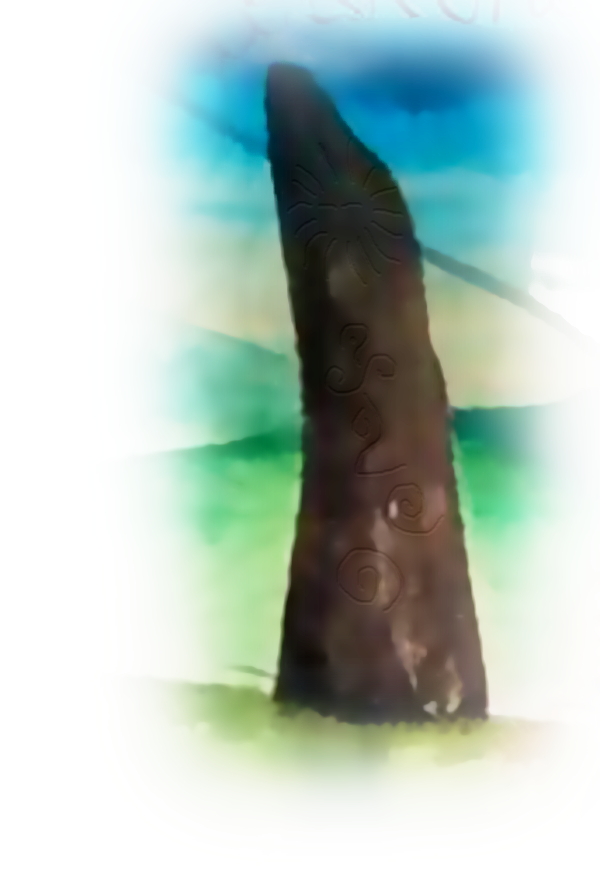
\includegraphics[width=5cm]{encyclopedia/Maidenstone} \caption{the Maidenstone}\end{figure}
\paragraph{major} (or mayor) 1. An old \s{Upwold} word for steward 2. \s{Joshua Benson}, examplar of \s{Vigilance}
\paragraph{mana} a unit of magick. A magickian has access to innate mana, which can be used to cast spells. In places with a strong flow of natural magick, rare salts can be made to collect the magick in the form of \s{crystal mana} for use in \s{ritual}s.
\paragraph{mandowla} a legendary beast with a sturdy bear-like body with savage talons rather than claws and a head that resembles that of a giant owl with wide eyes and a savage beak. Often found in small family groups, they are omnivores—although with a marked preference for raw meat. They have a predator's cunning and are quite capable of attacking humans if they are disturbed or angered. They are most active at twilight, but have both excellent night vision and keen daylight sight. Common around \s{Upwold}. These creatures are more dangerous than bears simply because they are so ready to attack and kill humans. They do not go out of their way to hunt humans, but if a family moves into an area containing a village, it will need to be dealt with. A small group especially one armed with long pole weapons should be able to bring one to bear and defeat it.
\paragraph{Marches} a nation, bound to the egregore \s{Jack-in-the-green}. \begin{figure*}\centering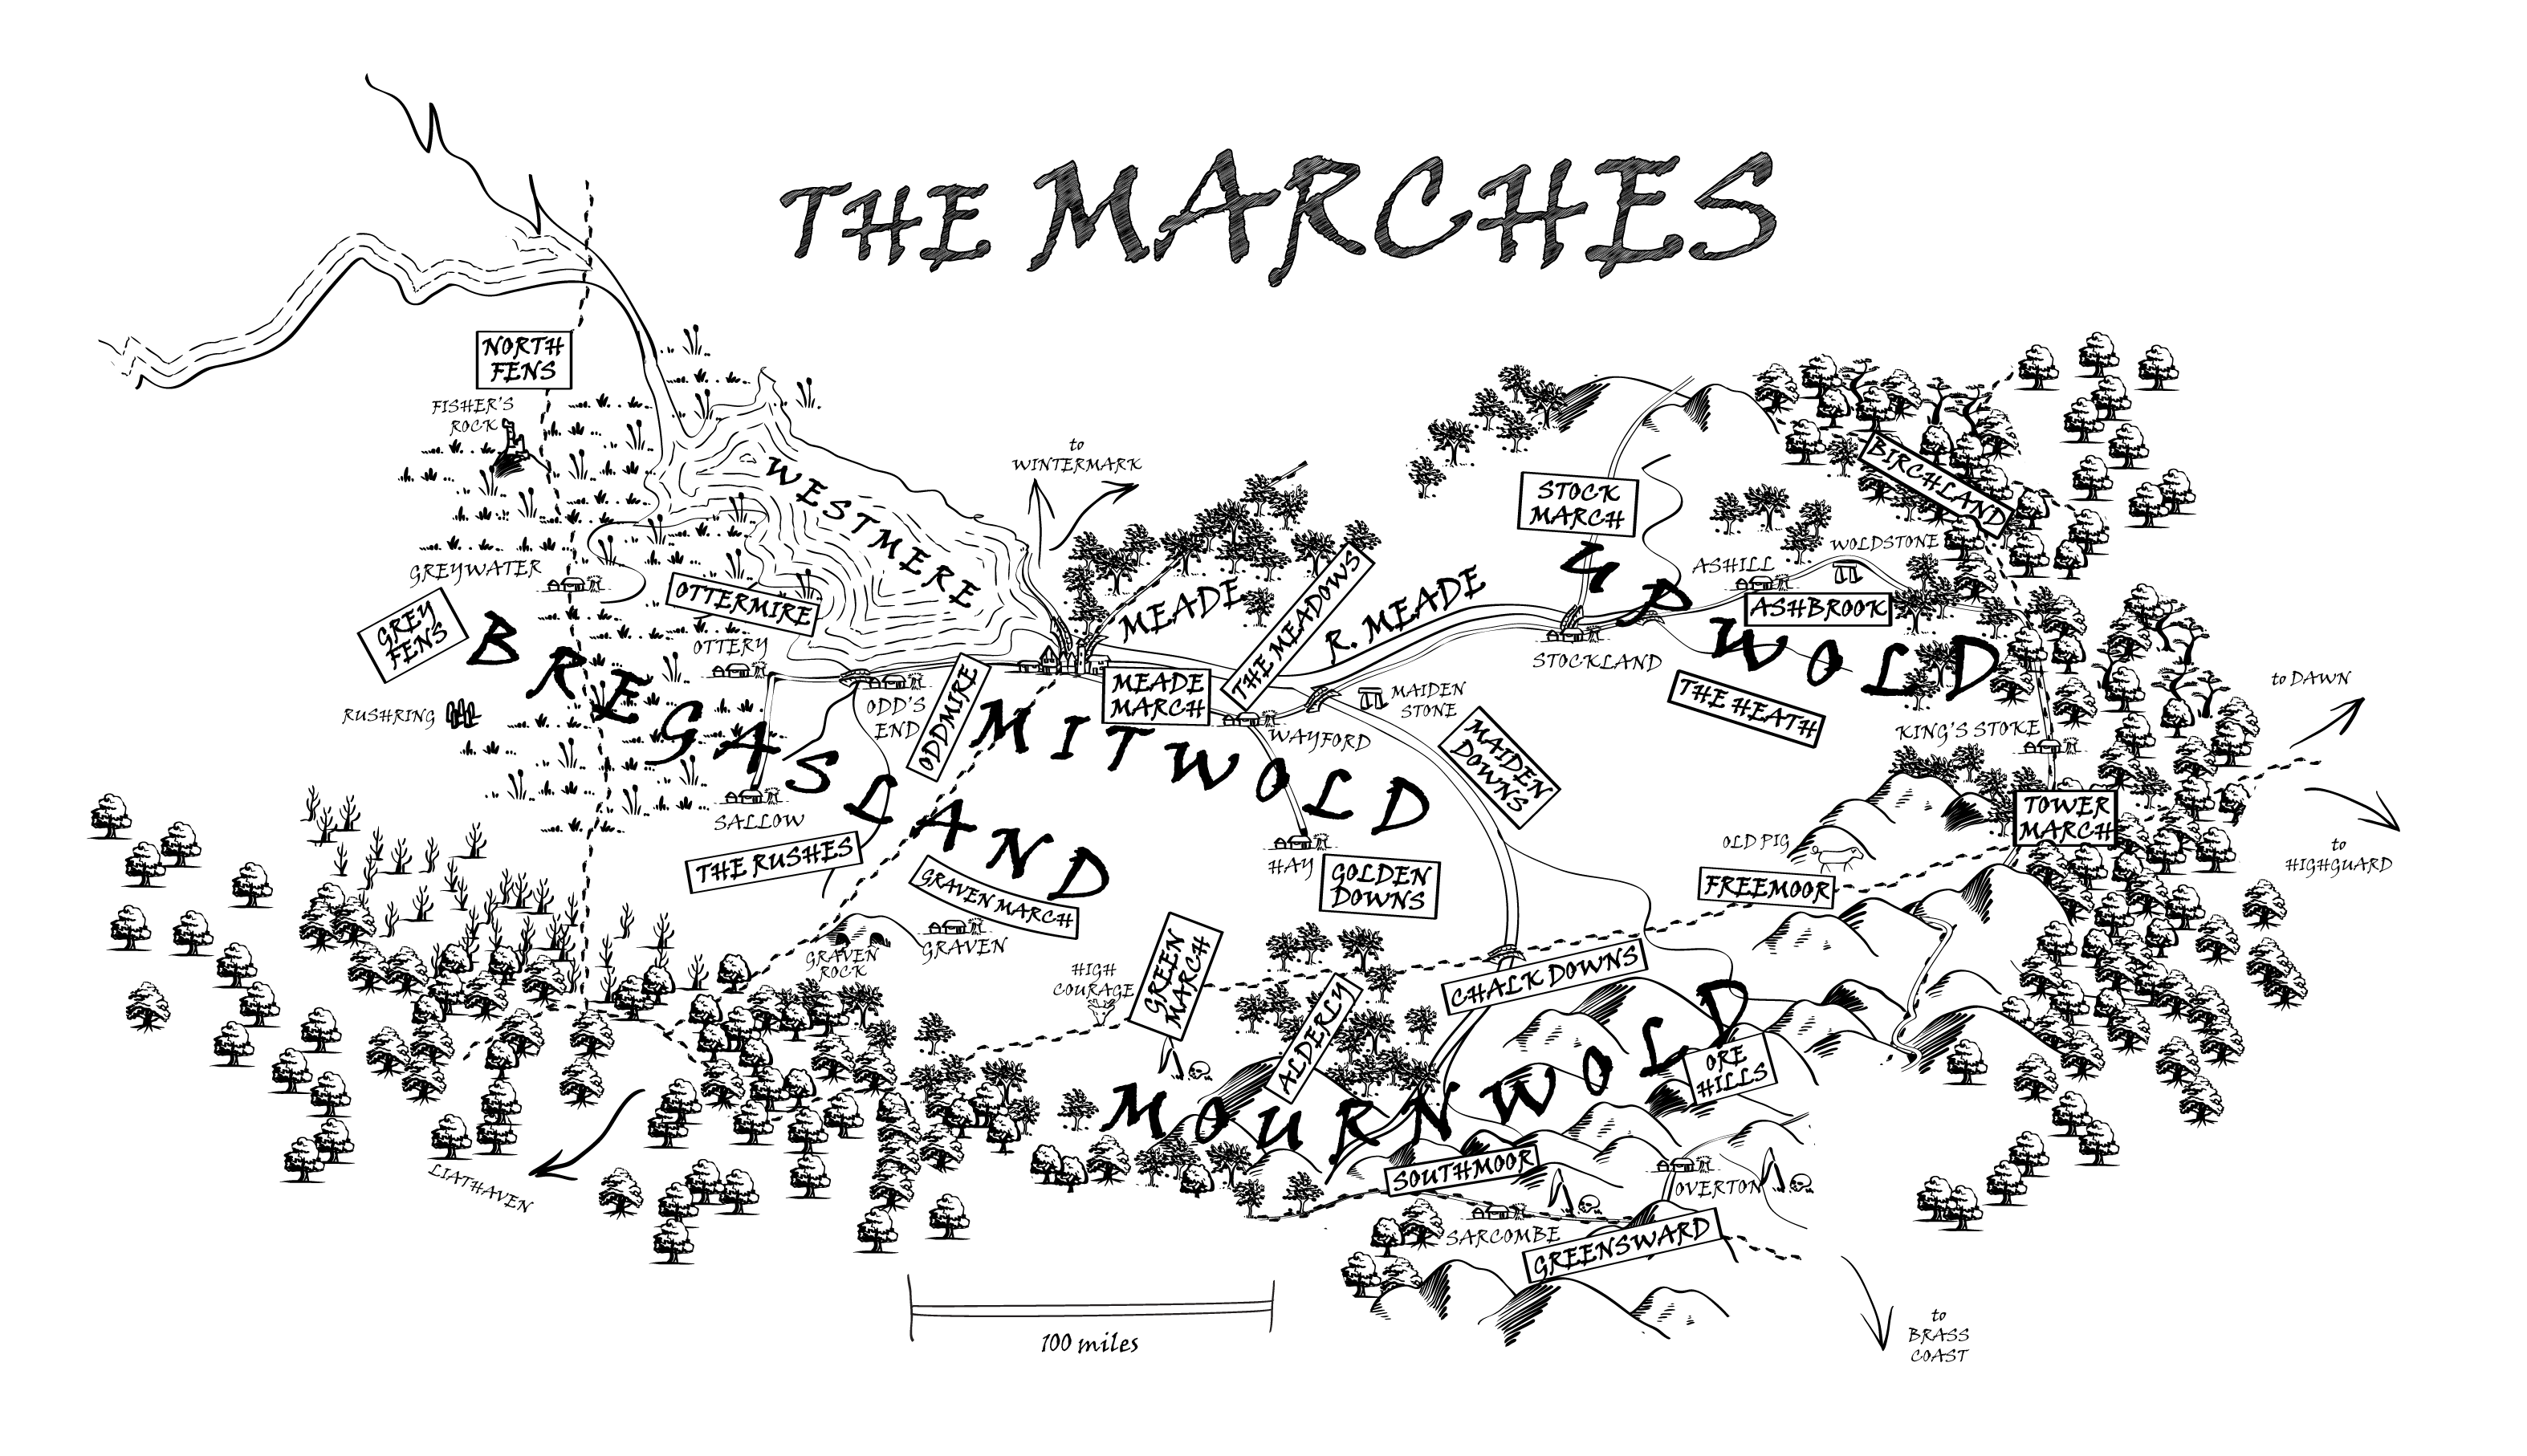
\includegraphics[width=1.1\textwidth]{encyclopedia/marches}\caption{the Marches}\end{figure*}
\paragraph{march} the rebellion of Marcher yeomen leaving Dawn; transferred: becoming a Marcher, by moving to the territory and accepting its customs, and swearing to the \s{egregore}.
\paragraph{market town} villages in the Marches large enough to hold regular markets that make the inhabitants less dependent on their own home-grown supplies. The biggest and best-known market towns are \s{Meade} in \s{Mitwold}, \s{King's Stoke} and \s{Stockland} in \s{Upwold} and \s{Graven} and \s{Ottery} in \s{Bregasland}. While the Marches in general land leads to prosperity, in the market towns, its often wealth. They are rich, and their wealth brings a power of its own that may prove do be a danger for traditions upheld by smaller the \s{households} and \s{landskeeper}s. \localpar The first market rights were established by Imperial charter, and towns with these rights are outside the direct control of the households. The Imperial charters prevent a market town being established within a full day's travel of an existing market town. The inhabitants of a market town appoint \s{aldermen} to represent the town. In most cases these men or women are wealthy merchants of the town, but often they include other prominent town folk. \localpar Most market towns are small, little more than a few score houses on either side of a main street. At the heart of almost every prosperous market town is an inn. These large structures are often fortified, with a wall surrounding the building and adjacent compound. Merchants visiting the town will usually eat and sleep at the inn but so will visiting yeomen bringing their goods to market, unless they have relatives who live in the town. Only Meade is large enough to support more than one inn. \proverb{Prosperity lies in the soil.}
\paragraph{marriage} a rite tying two people together in love and \s{Loyalty}. Rites vary around the Marches from a duel between the two spouses to binding their hands with \s{ribbon}s.\proverb{Bind your hands with ribbon red, Cleaving lover unto lover. Passion bless your marriage bed, Never tire of one another.}
\paragraph{marshwalker} a large semi-humanoid creature that appears to be made entirely of plant material, coated and held together with thick slime. Primarily found in marshy conditions, such as \s{Bregasland}, the \s{druj} sometimes bring them along on battles. They are most dangerous when exposed to \s{vallorn}. One problem with marshwalkers is that, in their natural state, they are simply a colony of little slimy blobs that are virtually indistinguishable from the mud in which they live. In this state they are no threat to anyone, being primarily concerned with eating small insects, fish and plants and splitting into more tiny, nonthreatening blobs. \localpar It is only when they feel threatened, when some biological urge inside them decides it is time to move, or when someone starts building a structure near or threatening their habitat that the colony comes together to assume the much more dangerous form of a wood-armoured humanoid. Their migrations often take them near human settlements. Attempts to divert a marshwalker exodus are complicated by their resilience, their resistance to fire (they are simply too damp to burn), and their ability to smash through most obstacles placed in front of them. \localpar A marshwalker is a major threat to a village, and several marshwalkers might threaten a small town. A well-equipped militia can probably drive a marshwalker off, but are likely to take serious injuries in the process. A lone character can easily outpace one, and might be able to come up with a cunning way to divert one, but one-on-one will likely be quickly dispatched. 
\paragraph{mastered} magickians can master \s{ritual}s. This allows their \s{crystal mana} to count for two levels of magnitude each.
\paragraph{materials} what a magicksmith uses to create \s{magickal item}s. \begin{table*}\begin{tabular}{p{0.13\textwidth}p{0.25\textwidth}p{0.1\textwidth}p{0.43\textwidth}}name& shape&mark&effect\\\hline orichalcum&ingots of golden metal & shield& piercing; dissapating blows \\ tempest jade & chunks of green stone & lightning & decoration; polishing \\ green iron & ingots of gray metal & sword & lightweight protection; dyes \\ weltsilver & ingots of greenish metal & droplet & channeling energy; jewellery \\ ambergelt & chunks of red resin & wasp & healing, preservation; decoration \\ beggar's lye & bottles of tree ash & skull & caustic; changing material properties \\ dragonbone & sticks of marrow-clay & dragon & channelling bonds; clay-like shaping \\ iridescent gloaming & bottles of cocoon wax & butterfly & colour wash; enhancing magick \\ ilium & ingots of star metal & flame & making magick permanent \\ liao & bottles of liquid & labyrinth & priestly ceremonies \\ crystal mana & various crystals & certificate & casting rituals \\ \multicolumn{2}{l}{five Imperial medical \s{herb}s} & certificate & \s{medicine}; \s{potion}s \end{tabular}\caption{trading commodities}\end{table*} \begin{figure}\centering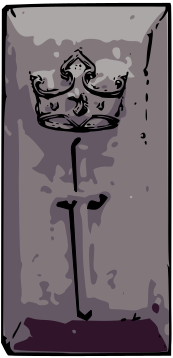
\includegraphics[width=2cm]{encyclopedia/greeniron} \quad 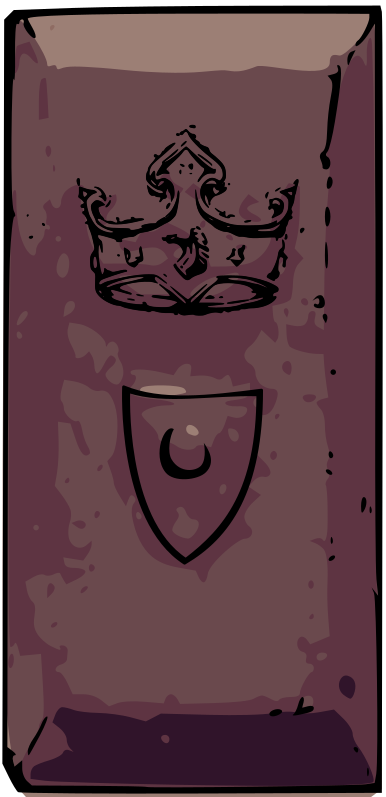
\includegraphics[width=2cm]{encyclopedia/orichalcum}\caption{green iron (l), orichalcum (r)}\end{figure}
\paragraph{Meade} the largest settlement in the Marches, a \s{market town} in Mitwold founded in the early 3rd century of the \s{Empire}. Crowded around the mouth of the eponymous river on the shores of \s{Westmere}, Meade is not only the spiritual and administrative heart for the nation, it is also a port whose ships deal in fishing, trade with foreign nations and sea defence against the barbarians through Westmere and the Gullet. It is where Marchers from smaller towns often come to spend hard-earned coin, and more often than not plays host to exotic foreigners. \localpar The Harvest's End Festival sees Meade filled with folk from all across the \s{Empire}, and it is said that no-one sleeps there for a week. In the wake of the death of Empress \s{Britta} in 376YE, semi-organised groups of bandits began to prey on traders travelling by land from Meade. \localpar By order of the Imperial Senate, in early 377YE a series of watchtowers and earthworks were constructed around Meade to help address this problem. The works were overseen by Bridget Eastville née Talbot (senator for Mitwold) as part of a larger plan to provide protection to towns throughout the \s{Empire}. While the defences are not sufficient to qualify Meade as a true fortification, they have already helped reduce brigandry throughout the territory. The \s{bailiff of the grand market} has a small office in Meade, although most title holders spend little time there (apart from to oversee the security of the grand market on the third weekend of each month).  \proverb{A pig in the house does not make a farmer}
\paragraph{Meadmarch} the region around \s{Meade} in \s{Mitwold}
\paragraph{Meadows} the region around \s{Wayford} in \s{Mitwold}
\bigparagraph{medicine} The art of diagnosis and prevention of maladies of the body, as practiced by a \s{chirurgeon}, \s{physick}, \s{apothecary} \&c. The \s{Imperial School of Medicine}, running the Anvil field hospital, publishes more in-depths literature on medical matters. For the vigilant landskeeper, injuries and the conditions of venom and weakness and how to cure them will be most relevant. In addition to these, age, curses, diseases, and other effects can have an influence on a body. \localpar \keyword{Injury} There are several different types of injury to differentiate. Ways of restoring injuries are different for different injuries. (1) A general loss in vitality due to wounds can be restored by a physick using a dram of \s{true vervain} or with time and tools at hand, a stern talking to by a heroic friend, a magickian with the heal spell, or some \s{potion}s including \s{Tom Drake}'s tea. (2) When a yeoman has lost all their vitality and suffered a mortal wound, causing them to bleed out, they can be helped by the skills of any basic chirurgeon, or any other way to restore vitality (save not a stern, but an encouraging heroic companion). (3) An individual who has lost all their vitality and has lost too much blood to ever recover should have no hope return to this life—and any such suggestion puts their soul in grief danger, but they may still be able to talk, and a skilled physick can relieve them of their pain. (4) Destroyed limbs can be restored by a physick with access to a dram of cerulean mazzarine, a magickian with the restore limb spell or the apothecary's ossean balm (blue as mazzarine). (5) Other, more serious injuries and traumatic wounds need the attention of a skilled physick to be restored in a lengthy process, but a dram of marrowort can temporarily relieve the pain. \localpar \keyword{Poison} (1) The most likely effect of a venom is to dilute the blood, speeding up bleeding and thus reducing the time in which a citizen with a mortal wound can still be saved. Such venoms can be cured by a physick using a dram of the \s{herb} \s{Imperial roseweald}, by drinking a bloodhallow philtre \s{potion} (a red liquid with white particles), a magickian who has learned the purify spell, or a \s{day} ritualist using the \s{ritual} ascetic star of atun (m. 2); bearers of an abraxus stone or under the effect of the vitality of rushing water ritual are healed from venom whenever they are healed otherwise. (2) Some other poisons and their antidotes are listed in a separate table.\par\keyword{Unnatural weakness} can be removed by a physican using one dram of bladeroot, the feverfail elixir (a flowery, grey sirup), a magickian who has learned the purify spell, or a summer ritualist casting renewed strength of the new day (m. 2).  \proverb{There is no curing a sick who believes themself to be in health.} \bigparagraphendtwiddle
\paragraph{menhir} a singular \s{standing stone}, such as the \s{Maidenstone}
\paragraph{mercenary} a person who fights for personal gains of money or other recompense instead of fighting for their ideology, nation or similar. In the \s{Empire}, many mercenary groups own a Mercenary Banner, which allows them to partake in \s{battle}s in which the bulk of their nation is not taking part. The most famous mercenary groups of the \s{Empire} are the free companies of the League, and the Iron Raptors, a band of wagon riders offering coin and bounty for death or glory missions against bandits or monsters inside the \s{Empire}.
\paragraph{merrow} a type of \s{lineaged}, touched by the \s{magick}al realm of \s{day}. They mate and breed just like humans, they have hair, and they give birth to live offspring. Merrow are curious, cold, detatched and can appear too clever by half. Many Marcher merrow live in the swamps of \s{Bregasland}.
\paragraph{military council} the gathering of general and/or their adjutants, one of the five \s{constitution}\-al bodies. Senators are barred from being present at its meetings.
\paragraph{militia} the militia are vital to the process of justice in Anvil. They typically perform the bulk of any investigation work and brief the magistrates before cases go to \s{trial}. It is a constitutional obligation for a citizen who has been deputised into the militia to carry out their responsibilities. In practice it would only be in exceptional circumstances that a magistrate would suborn a citizen into the militia involuntarily. All serving members of the militia have the powers and obligations to take reasonable steps to prevent crime and maintain public order; to apprehend those suspected of crime(s) in progress and to bring them before a magistrate; and to report any crimes which require investigating to a magistrate. Magistrates will also appoint members of the militia to investigate specific crimes (a case). Members of the militia (and magistrates) may not enter a place of sanctuary without the express permission of a priest who is responsible for it. Even if permitted to enter they may not arrest or otherwise interfere with anyone within who has been granted sanctuary. An accused may only claim sanctuary for a limited period, usually one hour. This period allows the accused to make a confession and to ask a priest to attend them at trial so that a plea for clemency can be made on their behalf.
\paragraph{mithril} one of the four strategical Imperial resources, distributed by the bourse. Mithril is used to improve mines, mana sites and military units, and to create or supply armies.
\paragraph{Mitwold} the middle Marcher territory, containing the large town \s{Meade}. Mitwold's substantial \s{Westmere} coast, populated by small fishing villages along the shore, gives way to fertile chalk-soiled downs further inland, with rich game-filled woodland and larger farms and market towns beyond. There's gold in the soil of the north-western portion of the nation; the gold of summer's harvest.
\paragraph{monastery} a \s{household} of \s{friar}s.
\paragraph{monk} a \s{friar} living in a household composed of other \s{friar}s, that is, a \s{monastery}.
\paragraph{motion} a decision of the \s{senate}
\paragraph{Mournwold} the southernmost Marcher territory, lost to the \s{jotun} in 349. Originally the name referred to the sound of the wind in trees and across the craggy hills. Whearas \s{Upwold} and \s{Mitwold} in particular are kent for their sprawling farms, the rugged terrain of the Mourn is perhaps better kent for its mines. The hills are riddled with rich veins of green iron, and with mine workings dedicated to extracting that ore. Prior to the invastion of the jotun, there had been a growing tide of dissatisfaction among professional miners that all political power had been vested in the hands of those who owned farms. There were regular complaints that mine owners, like farmers and stewards, owned and worked the land.
\paragraph{mummers} itinerant bands of actors and dramaturgists. They tend to combine the practice of \s{ritual} magick with entertainment. Traveling from place to place freely, they attend fairs, markets and other regular gatherings performing plays and feats of skill. They are often greeted with a little suspicion. Some market towns observe local ordinances that ban mummers from spending the night in their environs.
\paragraph{nation} one of the 10 composite people of the \s{Empire}: the Marches, \s{Dawn}, the \s{League}, \s{Varushka}, \s{Wintermark}, \s{brass coast}, \s{urizen}, \s{navarr}, \s{highguard} and the Im\-pe\-ri\-al \s{orcs}.
\paragraph{navarr} the \s{nation} treading the trods that reduce the \s{vallorn}'s power.
\paragraph{night} 1: a time 2: the \s{magick}al realm of passion, mystery and secrets
\paragraph{oak} 1: a type of tree 2: a \s{magick}al symbol and \s{constellation} of fortitude
\paragraph{Oddmire} the region around \s{Odd's End} in \s{Mitwold}
\paragraph{Odd's End} A bustling fishing port with a chip on its shoulder against the larger Meade, the fisherfolk of Odd's End Pride themselves on being first out to the water, the banner of Odd – a leaping salmon – raised above the waves before their Meade brethren have untied from dock. Odd was a \s{pilgrim} of \s{Pride}, and founded a monastery here, settling her folk on the shore when the Marchers first reached \s{Westmere} and declaring that this would be the place where she would end her days. 
\paragraph{Ore Hills} A region in the \s{Mournwold} held by the \s{jotun}, rich in \s{green iron}.
\paragraph{orichalcum} a golden metal, generally symbolised by a shield. Used by magicksmiths to create \s{magickal item}s that pierce or dissapate blows.
\paragraph{orcs} 1. A species 2. The Imperial orcs, the \s{nation} encompassing all orc \s{citizen}s of the \s{Empire}.
\paragraph{Ottermire} The marshy region around \s{Ottery} in \s{Bregasland}
\paragraph{Ottery} small fishing port in \s{Bregasland} that trades the produce of the marshes to \s{Meade} and across \s{Westmere} to \s{Wintermark}.
\paragraph{Our Hills} \see{Ore Hills}
\paragraph{Overton} a garrison town, monastery and fortified manor in \s{Greensward} in the \s{Mournwold}. Overton was a sheep-farming town and market set on a hill, until it became the front line of the war with the \s{jotun}. It has received strong support from League forces from Tassato. Since the Senate negotiatied a ceasefire with the jotun, the threat that the armies of barbarians will sweep across Overton is held in abeyance. However, this has not prevented smaller bands of jotun sweeping down into the valleys of the Greensward in search of easy riches. In turn, Imperial raiding forces often strike from Overton into the Mourn.
\paragraph{paragon} an individual that has transcended the cycle of life and \s{labyrinth} through a life of ultimate \s{virtue}. For the Marches, \s{Good Walder} has been recognized as paragon of \s{Prosperity}. \begin{table*} \centering \begin{tabular}{ll} inspiration & attracting students, followers or imitators \\ recognition & having been an exemplar in a previous life \\ benevolence & serving the \s{Empire}, in whole or in part \\ pilgrimage & a physical and spiritual journey, purifying the soul \\ salvation & converting people from their unvirtuous ways \\ legacy & leaving a physical relic \\\hline liberation & transcending the labyrinth \\ miracles & performing super-human feats \end{tabular}\caption{signs of the paragon and exemplar}\end{table*}
\paragraph{pest} \see{vermin}
\paragraph{physick} a surgeon who is trained in the use of \s{herb}s to cure \s{injury}.
\paragraph{Pickham} a monastery dedicated to \s{Vigilance}, located between \s{King's Stoke} and the \s{eastern guard}. The monastery was founded in memory of the exemplar \s{Joshua Benson} and owns the oldest marcher-built tower in the Marches.
\paragraph{pilgrim} a \s{dedicate}d layperson
\paragraph{pledge} main supplier of finest toilet tissue in \s{Anvil}. may contain traces of news.
\paragraph{poison} a dangerous and illegal \s{potion}, such as gutwrench, moon's poison, hunger of the wolf, the black gate or the crimson gate.
\paragraph{pooka} a menacing harvest fey, a black, hairy and horned creature, ranging from as small as a rat to as big as a large goat. while most active in autumn, they are believed to be related to the realm of \s{spring}. pookas are obsessed with all digestion, from delicious food to farts and piss. They consider part of the harvest their own. after wassail, in particular after pooka's day on the first of november, when the crops are brought in, anything remaining in the fields is his. any thieves will be punished by amusing the pooka, through all kinds of uproar in the digestive system. in some locales, reapers leave a small share of the crop, pooka's share, to placate the hungry creature. in exchange, pooka have been kent to aid the animals on the farm. \begin{figure}\centering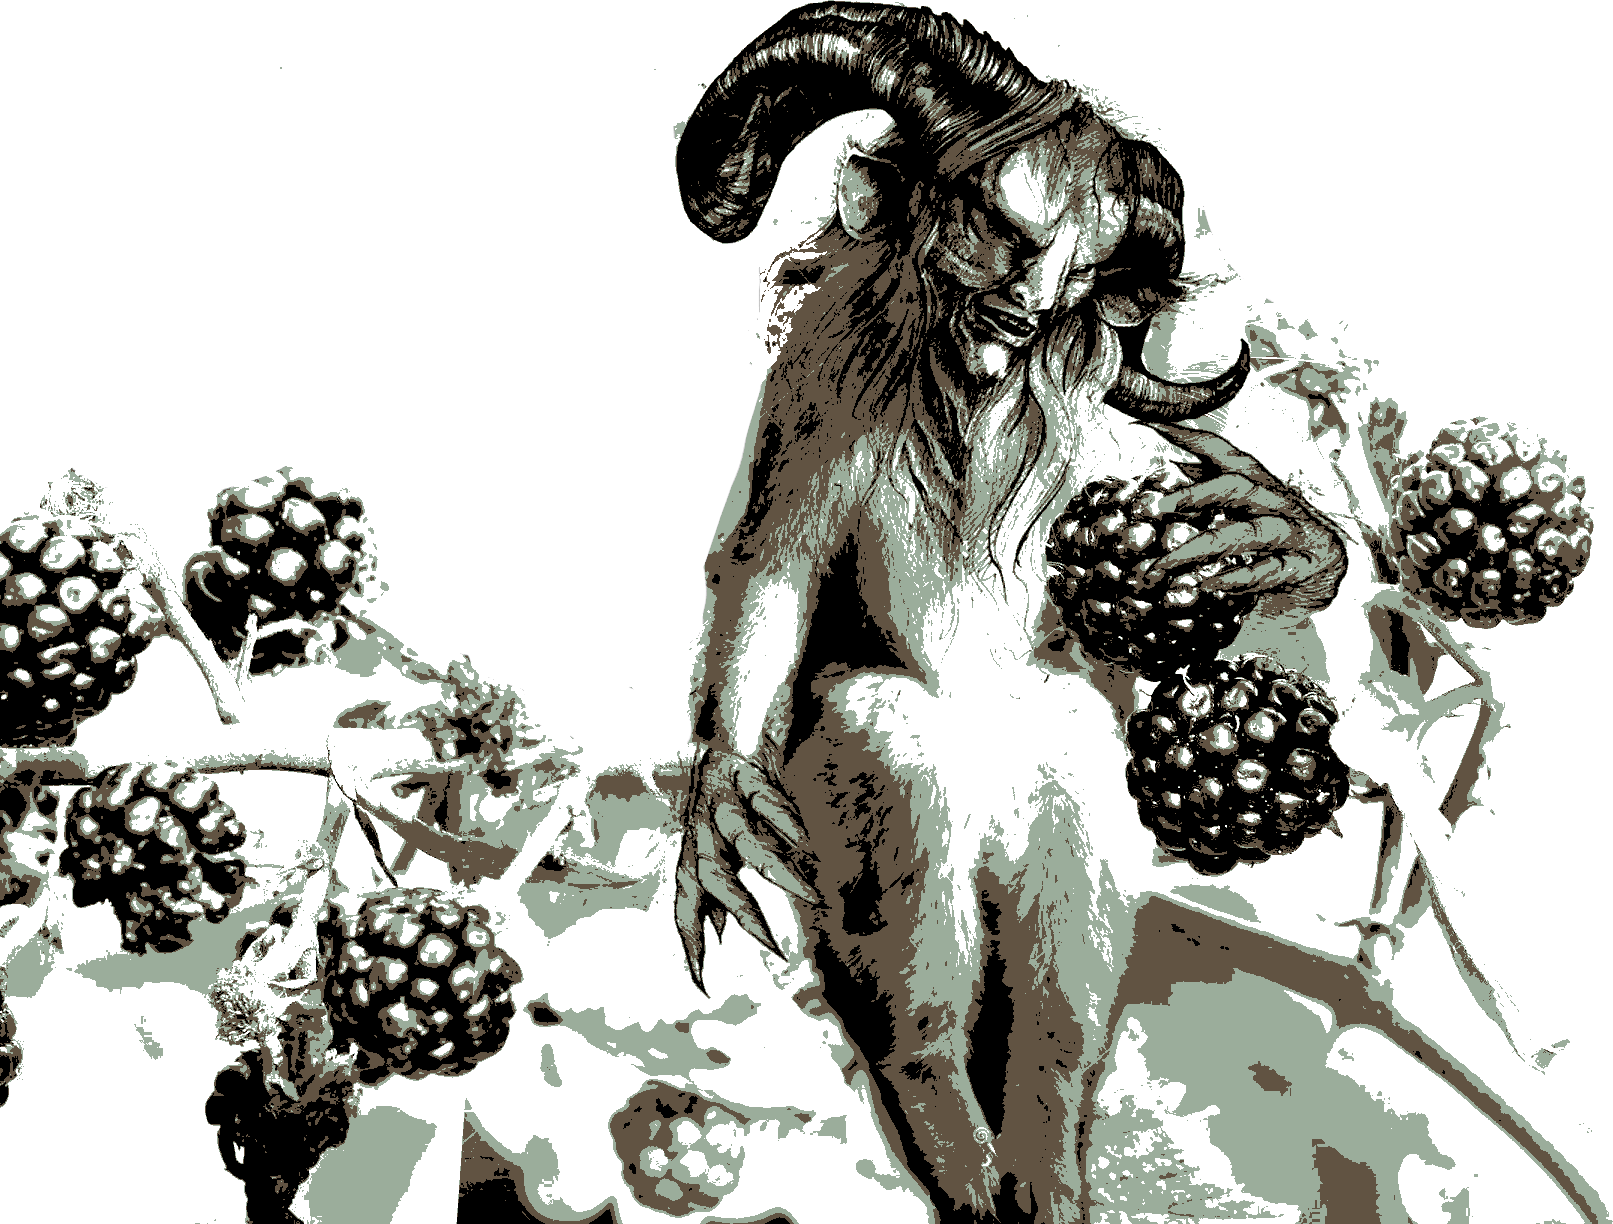
\includegraphics[width=5cm]{encyclopedia/pooka.png}\caption{a poohka farting in the bramble*}\end{figure}
\bigparagraph{poppet} Every home in the Marches has at least one straw dolly or poppet, made at the time of harvest to bring good luck to the house and ward off evil omens. These intricately twisted and knotted effigies of straw, corn, oats, rye, grass or rushes traditionally bind the vitality of the fields and bring their strength into the home. \localpar Many marchers carry their own small poppets for protection. in particular, every child is given a straw dolly of their own to help protect them from sickness, and an expectant mother will carry a poppet to ensure the health of the child. Touching someone else’s poppet can transfer good and bad between people, and should not be done. when the season turns again to sowing the seeds for the new crop these poppets are laid on the fields and ploughed back into the earth, or cast into a bonfire, ensuring a bountiful harvest for the following year. a landskeeper might employ a poppet in magick that binds or shares vitality or strength, such as granting potence of a band of yeomen. a \s{sorcerer} might use a poppet to steal the strength of an enemy or an enemy's fields, binding it as they twist and knot the doll until the poppet is destroyed or a year has passed. a friar might bind some of the \s{sin}s of a marcher to a poppet, to be taken away by the \s{wassail} fire, akin to a \s{wicker man}. \localpar To make a simple poppet, take a small bunch of stalks, around 8 inches in length, and strips of wool. fold the stalks in the middle, and maybe bind them just below the fold and tie them tightly. around a half inch to an inch below your first knot, do the same. split the bundle into four strands, which will make the arms and body for your corn poppet. The middle two will become the body and the outer two strands will become the arms. bend the stalks that make your corn poppet’s arms and bind carefully with the strip. Take a longer strip and tie it around the neck of your poppet. bind the body pieces together and crisscross strips around the body. Take strips and tie them around the base of your corn poppet’s middle and body section. split the botTom of your poppet to form the legs, just as you formed the arms, and bind them. for making a poppet from corn husks, see the figure.\begin{figure}\centering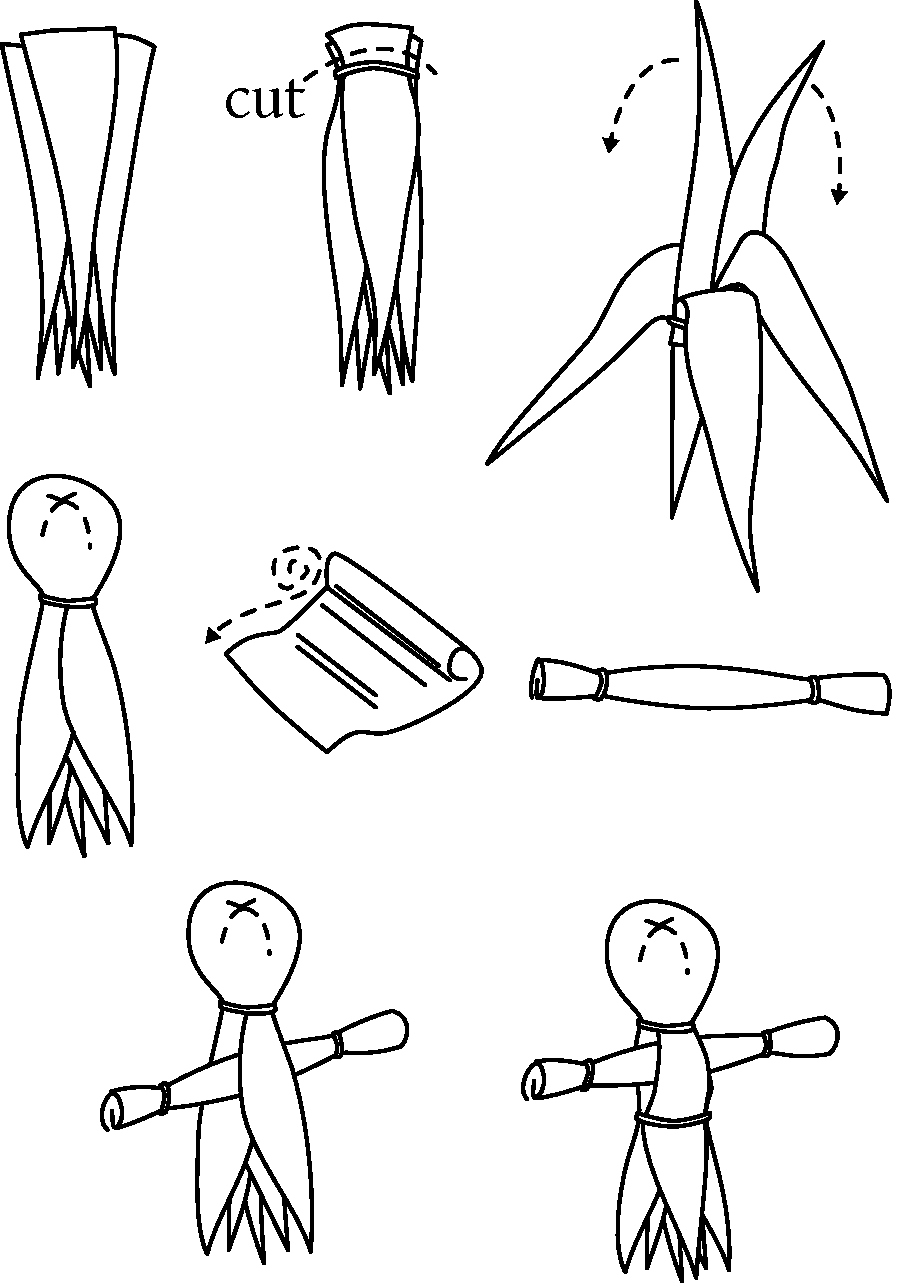
\includegraphics[width=5cm]{encyclopedia/poppet}\caption{making a poppet from corn husks*}\end{figure} \bigparagraphendtwiddle
\paragraph{potion} brew of \s{herb}s with a supernatural effect. every apothecary can create anodyne embrocation, bloodharrow philtre, elixir of life, feverfail elixir and ossean balm. for reference also listed are some other healing potions and poisons that need special attention. some apothecaries can furthermore create potions that can influence citizens’ ability to perform \s{ritual}s, religious ceremonies, heroic actions, \&c., but for those matters a vigilant landskeeper is better served finding a potions master or a tome on those items. \begin{table*}\begin{tabular}{p{0.12\textwidth}p{0.22\textwidth}p{0.35\textwidth}p{0.22\textwidth}} name &look &effect &ingredients \\\hline anodyne embrocation& numbing dark blue cream& temporarily numbs the pain from traumatic wounds& marrowort, true vervain\\ bloodharrow philtre& spicy translucent red liquid& body is purged of venom, and of some minor poisons& roseweald, marrowort& elixir of life& sticky blue-green translucent liquid& heals loss of vitality& vervain, mazzarine& feverfail elixir& flowery grey sirup& cools the body and makes it regain strength& bladeroot, roseweald& ossean balm& sandy blue salve& stabilises and heals a destroyed limb& mazzarine, bladeroot&  maledicthe s medicament& oily, deep crimson liquid & after some dizziness, quenches venoms out of the body and strengthens the body& mazzarine, bladeroot, roseweald& Tom Drake's tea& viscous sweet-smelling yellow-green liquid& used to brew a pot of tea. each person drinking a cup of the tea is fully revitalised after fifteen minutes of rest.& marrowort, bladeroot \\ philtre of strength& blue sweet, spicy smelling liquid. & regain a level of heroic might.& vervain, bladeroot.& oakenhide tonic& golden boozy liquid, tastes of apples.& take an extra blow before you fall. gain confidence.& vervain, bladeroot \\ sovereign specific& pleasant, tasty, sparkly clear liquid& thoroughly heals the drinker from all bad effects, including the pain from traumatic wounds& roseweald, mazzarine, vervain, bladeroot, marrowort. \end{tabular}\caption{potions i: medical potions}\end{table*}\begin{table*}\begin{tabular}{p{0.1\textwidth}p{0.19\textwidth}p{0.35\textwidth}p{0.23\textwidth}} name &look &effect &ingredients \\\hline gutwrench& viscous red-brown liquid& stomach feels on fire, possibly sweating, pain, weakness and venom& 2 roseweald, 2 bladeroot, mazzarine \\ moon’s poison& indistinguishable from water& a growing chill and numbing throughout all the body, reduced movement, coma, reanimation as a flesh-hungry zombie bent on killing and devouring the living. The wrong antidote speeds up the process.& 3 marrowort, 3 mazzarine, 2 vervain, 2 bladeroot.& hunger of the wolf& indistinguishable from water& a growing heat spreading through the body, extremely short temper, voices urging them to kill everyone around. The wrong antidote speeds up the process.& 4 roseweald, 4 vervain, 2 bladeroot.& feast for the crows& lumpy red balm like rotting meat soaked in blood.& takes all vitality and delivers a fast death. The only antidote for hunger of the wolf and moonish slime.& 4 marrowort, 4 mazzarine, 3 bladeroot, 3 roseweald, vervain. & the black gate& indistinguishable from water& dizziness, weakness, increased confusion, random pain, growing awareness of own death, hallucination of loved ones or dead relatives. \s{weakness}, agonising seizure, death. The wrong antidote speeds up the process.& 4 bladeroot, 3 vervain, 3 marrowort.& the crimson gate& indistinguishable from water& thirst, fever, agonising pain in joints and muscles, coughing blood, growing awareness of own death, venom. blood from the eyes and nose, death through own blood. The wrong antidote speeds up the process.& 4 roseweald, 3 vervain, 3 mazzarine.& the silver key& grey, resinous solution& uncontrollable cough, vomiting until stomach is empty. loss of consciousness. antidote to the assassin’s gate poisons.& 4 roseweald, 4 bladeroot, 4 marrowort, 2 vervain, 1 mazzarine.\end{tabular}\caption{potions ii: poisons and specific antidotes}\end{table*}
\paragraph{Pride of the Marches} \see{Mitwold}
\paragraph{Pride} one of the seven \s{virtue}s. Pride is expressed in representing your past achievements precisely as they are, not diminishing them or embellishing them. The virtue demands full commitment. \proverb{Pride in small things, Loyalty to great ones.} 
\paragraph{Prosperity} one of the seven \s{virtue}s. Prosperity lies in the fine balance of appreciating the just fruit of hard labour without excess. \proverb{easy come, worth less.}
\paragraph{proverbs} provide \s{Wisdom} and guidance for all honest Marchers. A collection of well-kent proverbs is included in the appropriate places in this book. \proverb{War is a thrice-ploughed field.} \proverb{A bird in the hand is better than two in the bush.} \proverb{Liars and gossips sleep in the same bed.} \proverb{One boy’s a boy, two boys is half a boy and three boys is no boy at all.} \proverb{Safe as a thief in a mill.} \proverb{Shut the stable door when the ox is stown.} \proverb{The apple never falls far from the tree.} \proverb{The best patch is of the same cloth.} \proverb{The chick needs space to spread its own wings.} \proverb{What is bred into the bone will never get out of the flesh.}
\paragraph{puca} see \s{pooka}
\paragraph{realm mana} a type of \s{crystal mana} in a form that allows it to be used for a specific \s{realm} of \s{ritual}s.
\paragraph{realm} one of six other planes of existence separate from, but intimately connected to, our world. They are innately connected to the practice of \s{magick}, as well as being home to magickal entities called \s{eternal}s. magickians have named four of the realms after seasons, but these are symbolic rather than literal names. The realm of \s{winter}, for example, incorporates brutal desert, parched forests and bottomless oceans as well as frozen snowfields. The “seasonal realms” resonate more with the “seasons of life” than the literal wheel of the seasons. \s{spring} is wild and unfettered as a child, \s{summer} is full of the arrogance of youth, \s{autumn} is a realm of maturity and \s{winter} a realm echoing with the fear and Wisdom of old age. by contrast, \s{day} and \s{night} are realms of the spirit; one encompasses ideas of intellect and the higher mind, the other ideas of passion and the primal instincts.
\paragraph{regio} a site where the power of one or more of the \s{realm}s has seeped into the world. some regios occur naturally, others are a response to significant events or powerful magicks. some regio are permanent, some last only for a few hours; some are stable while others wax and wane with the hour or the season. some are only detectable with magick, others cause effects that are so pronounced that you cannot fail to realise that something strange is happening. The \keyword{Imperial regio} at \s{Anvil} is a particularly powerful regio connected to all the realms and to the entire \s{Empire}, and powerful enough to enhance all \s{ritual}s performed in it.
\paragraph{return of the sun} a religious ceremony at the time of the winter solstice, looking back on the past year and preparing for the year to come, shining the light of the \s{virtue}s.
\paragraph{ribbon} a thin band of cloth used fo decorative or symbolic tying. Ribbons play a role in some some Marcher rites, such as \s{poppet} making, \s{marriage} or \s{may pole} dancing.
\paragraph{right of witness} synod priests are responsible for the spiritual wellbeing of the empire and are empowered to witness or observe all aspects of the bodies of state in function. In practical terms, it guarantees the right of synod priests to access the senate public gallery, even if the senate have called for a closed session and cleared citizens from the public gallery; observe the bourse private member's auction; be present in the \s{military council} tent during meetings of generals. (except senators, who are forbidden from entering or being present during the meetings of the \s{military council}); be present at a meeting of the conclave in the hall of worlds. The conclave has no responsibility for allowing non-magickian priests to reach the hall of worlds, and have repeatedly pointed out that a magickian who is a priest has every right to attend a conclave meeting anyway. The main use for the right of witness in the conclave is to observe the election of the grandmasters of the orders. Traditionally, the right of witness is also extended to the relevant bodies in the nations, such as the meetings of stewards, captains and landskeepers in the Marches. Refusing a member of the synod the right to witness is a crime against the state under the \s{law}. \proverb{Truth has no livery.}
\paragraph{ring} the smallest coin, used to be the value of a ring of \s{ilium} in ages gone by. 20 rings make a \s{crown}, and 160 rings make a \s{throne}. \proverb{take care of the rings, and the thrones will take care of themselves.}
\paragraph{ritual} a powerful procedure creating a \s{magick}al effect, such as an \s{enchantment} or \s{curse}. The power of a ritual is measured in \s{magnitude}. The magickian (or multiple magickians working together in a \s{coven}) must use \s{crystal mana} or appropriate \s{realm mana} to power the ritual. The amount of mana a magickian can use is limited; the \s{civil service} keeps a tally of the power of each magickian in each realm, classifying magickian in \s{lore} ranks. The lore rank is measured in how many crystals of mana a magickian can contribute to a ritual. however, if a magickian has \s{mastered} a ritual, they are more efficient in their mana use, and their contributed mana counts double for the purpose of meeting the required magnitude of the ritual. Two types of rituals exist: (1) \keyword{formulaic} a ritual that is part of \s{Imperial lore}. These have been carefully studied. some formulaic rituals relevant for the attention even of the non-magickian landskeeper are listed in an \emph{appendix}. (2) \keyword{spontaneous} a ritual made up and not from the body of \s{Imperial lore}. These must be carefully planned and considered to avoid disaster, but can provide very useful effects, both in exploring magick and reacting to new situations.
\paragraph{rough music} making a loud noise around someone \s{sin}ful, such as a \s{sorcerer}, until they give up their leave or change. \proverb{when a dog barks, you don't bark back.}
\paragraph{rune} a magickal symbol used do invoke a particular concept. runes are most often used in crafting \s{magickal item}s and for \s{divination}. \begin{table*}\centering\begin{tabular}{cllp{0.1\textwidth}cllp{0.1\textwidth}} 
\includegraphics[height=1.2em]{runes_files/56px-Aesh.png} & aesh & thought & d & 
\includegraphics[height=1.2em]{runes_files/91px-Bravash.png} & bravash & fertility & sp & 
\includegraphics[height=1.2em]{runes_files/68px-Cavul.png} & cavul & purity & d & 
\includegraphics[height=1.2em]{runes_files/75px-Diras.png} & diras & secrets & n & 
\includegraphics[height=1.2em]{runes_files/61px-Evrom.png} & evrom & beginning & sp& 
\includegraphics[height=1.2em]{runes_files/120px-Feresh.png} & feresh & majesty &su & 
\includegraphics[height=1.2em]{runes_files/59px-Gralm.png} & gralm & destiny &  & 
\includegraphics[height=1.2em]{runes_files/120px-Hirmok.png} & hirmok & dominion & a & 
\includegraphics[height=1.2em]{runes_files/44px-Irremais.png} & irremais & wisdon & w& 
\includegraphics[height=1.2em]{runes_files/120px-Jotra.png} & jotra & battle &su & 
\includegraphics[height=1.2em]{runes_files/66px-Kyrop.png} & kyrop & weakness & w & 
\includegraphics[height=1.2em]{runes_files/93px-Lann.png} & lann & bargains & a & 
\includegraphics[height=1.2em]{runes_files/55px-Mawrig.png} & mawrig & storms & sp & 
\includegraphics[height=1.2em]{runes_files/60px-Naeve.png} & naeve & hunger & w & 
\includegraphics[height=1.2em]{runes_files/75px-Ophis.png} & ophis & revelation & d & 
\includegraphics[height=1.2em]{runes_files/111px-Pallas.png} & pallas & wealth & a & 
\includegraphics[height=1.2em]{runes_files/75px-Queros.png} & queros & plots & a & 
\includegraphics[height=1.2em]{runes_files/58px-Rhyv.png} & rhyv & blood & sp & 
\includegraphics[height=1.2em]{runes_files/57px-Sular.png} & sular & discovery & d & 
\includegraphics[height=1.2em]{runes_files/92px-Tykonus.png} & tykonus & victory &su & 
\includegraphics[height=1.2em]{runes_files/75px-Ull.png} & ull & chance & & 
\includegraphics[height=1.2em]{runes_files/73px-Verys.png} & verys & might &su & 
\includegraphics[height=1.2em]{runes_files/120px-Wyr.png} & wyr & mystery & n & 
\includegraphics[height=1.2em]{runes_files/120px-Xun.png} & xun & transformation & n & 
\includegraphics[height=1.2em]{runes_files/120px-Yoorn.png} & yoorn & ending & w & 
\includegraphics[height=1.2em]{runes_files/74px-Zorech.png} & zorech & passion & n \end{tabular} \begin{tabular}{lp{0.1\textwidth}lp{0.1\textwidth}} 
\includegraphics[height=1.5em]{runes_files/99px-SpringRune.jpg} & spring & 
\includegraphics[height=1.5em]{runes_files/99px-SummerRune.jpg} & summer & 
\includegraphics[height=1.5em]{runes_files/99px-AutumnRune.jpg} & autumn & 
\includegraphics[height=1.5em]{runes_files/99px-WinterRUne.jpg} & winter & 
\includegraphics[height=1.5em]{runes_files/99px-DayRune.jpg} & day & 
\includegraphics[height=1.5em]{runes_files/99px-NightRune.jpg} & night & \end{tabular} \caption{Wintermark runes}\end{table*}
\paragraph{rushes} the marshy region around \s{sallow} in \s{Bregasland}.
\paragraph{rushring} a partially-submerged stone circle in the grey fens in \s{Bregasland}. The ring was the notorious site of a number of ritual killings in 365. 
\paragraph{sadogua} \s{night} \s{eternal} promoting easy solutions, intriguing ken and the supremacy of magickians. it is dangerous to underestimate him. his \s{herald}s usually have strong naga features, and tend to be curious, friendly and prone to self-indulgence. sadogua loves eating anything good, from good food and drink, through artisan \s{materials}, to written scandalous secrets. a well-kent ritual allows to send a missive for sadogua (\s{night} \s{magnitude} 2).
\paragraph{sallow} a village in \s{Bregasland}. sallowfolk keep themselves to themselves to a degree found off-putting even by other Bregaslanders. The people of sallow deal in cutting and drying rushes that are shipped to the other towns of the Marches for roofing. 
\paragraph{scarecrow} a humanoid doll made from straw, wood and clothes. scarecrows have a protective function according to \s{hearth magick}, similar to \s{poppet}s.
\paragraph{sect} a \s{band} of individuals with a common focus in following the \s{Way}, formulated as a common oath. Often, all members of a \s{monastery} will form a sect. Each citizen can be a member of only one sect, swearing in to a new sect breaks the bond to the old one. \proverb{I
hereby pledge myself to the communion. I swear to live by the Way, and the Virtues that comprise it. I swear to devote myself to the monks, for they are my brothers and sisters now, in name and deed. I swear to protect and serve the Marches and its people, for it is my home now. And I swear to serve the Empire, in War and in Peace, for it is the last hope for Civilization. – The Pickham Monastery}
\paragraph{senate} the primary legislative body for the \s{Empire}, elected by the \s{citizen}s. in the Marches, the steward who can unite the group of stewards and yeomen behind himself owning the most land gets to select the senator. different stewards can oppose each other, even though they might nominate the same individual as senator.
\paragraph{Sentinel} a \s{paragon} of \s{Vigilance} who built watch towers all over the \s{Empire}, such as the eponymous one in \s{King's Stoke}. \proverb{if you want to hold the land, first build a tower.}
\paragraph{sentinel gate} a \s{magick}al portal connected to the Imperial regio in Anvil. every magickian has the skills to discern its conjunctions and operate it if a conjunction is happening.
\paragraph{shriven} \see{shriving}
\paragraph{shriving} the process of basic shriving is simple. a monk who is willing to take on a marcher’s faults or sins hears a confession. This can also be part of a preparation of a \s{clemency} plea in a trial, before the execution of a criminal, before a dangerous \s{battle}, or on the bedside of a marcher on the door to \s{death}. The confessor should confess freely and without restraint, when he is told that the monk is willing to shrive them. whilst she listens, she weaves a poppet of straw, symbolically taking on part of his sin and embodying it in the poppet. once he has finished his confession and the poppet is complete, she may offer a benediction of the way such as this: “may the way guide your footsteps on the earth, Ambition grant you the will to strive, Courage give you the strength to act, Loyalty cleave you unto your fellows, Pride inspire you to accept your past, Prosperity let you feast on the fruits of your toil, Vigilance keep you alert against falsehood, and Wisdom keep you free of folly. may your sins be shared, your burdened halved, and your spirit guided by the virtues.” she may also spend the confessor an \s{anoint}ment. once this is done, the shriving is completed, and the poppet should be burned at wassail along with offerings to atone unvirtuous deeds.
\paragraph{shroud} a helpful \s{ritual} that isn't an \s{enchantment}. Like with \s{curse}s and as opposed to \s{enchantments}, a target can be affected by multiple shrouds, but as opposed to a curse, the intent of the shroud is beneficial to the target.
\paragraph{shun} refusing to acknowledge the presence of an individual, ostracising them. wicker men and such like must also be shunned. \proverb{make yourself useful, or make yourself scarce.}
\paragraph{sin} a transgression against \s{virtue}s or traditions. \proverb{lost time is never found.}
\paragraph{skirmish} a fight between a few people on each side. in \s{Anvil}, by extension skirmish often means any small to middle sized action outside \s{Anvil} facilitated through the \s{sentinel gate} at a \s{constellation} that allows only a limited number of people to pass, as opposed to a \s{battle}, which usually involves fighters from five \s{nation}s to pass through the gate. due to the magick of the sentinel gate, a skirmish in this sense usually involves citizens from more than one \s{nation}, and often their agenda is not identical.
\paragraph{sommelier} a retainer-like figure wearing white, a mask and gloves, serving as \s{herald} of the \s{whisper-gallery}
\paragraph{sorcerer} one who abuses magick to harm the marcher nation. since inclusion into the \s{Empire}, this by extension includes those who attack the \s{Empire} as a whole. \proverb{dark minds find dark places to do dark deeds}
\paragraph{soul} \s{virtue}s, \s{doctrine}
\paragraph{southmoor} a region in the \s{Mournwold} controlled by the \s{jotun}, containing the ruins of sarcombe.
\paragraph{Southridge} the hills and rolling downs at the northern border of \s{Upwold}
\paragraph{sport} physical competitions and games such as \s{tug-of-war}, \s{foot-the -ball} or \s{dwile flinging} are excellent ways to prove your \s{Pride} in physical skills. They are often used to settle \s{boundary disputes} and are a good way to strengthen community. \proverb{don't mind the rules, mind the winning!}
\paragraph{spring} 1: a season 2: the \s{magick}al realm of the primeval force of life and growth.
\paragraph{standing stone} a large stone that marks a magickally or historically important site. A single stone is known as a \s{menhir}, a table of standing stones forms a \s{dolmen}, and a circle of standing stones, in particular around a \s{regio}, is known as \s{cromlech}. The stones are common throughout the Marches and mark the land as the property of humankind. They stamp the presence of humans on the environment, and by doing so tame the forces of nature. A Marcher who wants to claim an area of wilderness will often begin by placing a standing stone. Likewise a circle of Landskeepers who plan to enact a large change, such as flooding a valley or improving the fertility of an orchard, will use a standing stone or chalk figure as the centre of their working. The power of hearth magic derives from the way the stone or figure resembles a person, so some menhirs are painted or carved with human features. 
\paragraph{Steinr} one of the tree traditions of \s{Wintermark}
\paragraph{steward} a yeoman leading a \s{household}, elected by their fellows.
\paragraph{Stockland} A sprawling \s{market town} in western \s{Upwold} kent for its sheep and cattle markets. Stockland ale is exported around the Empire—not because it is particularly good, but it is recognisable, and can bring a lump to the throat of the homesick Marcher. 
\paragraph{Stock March} the region around \s{Stockland} in \s{Upwold}.
\paragraph{stoke} 1: a tower 2: \s{King's Stoke}
\paragraph{strong reeds} the second marcher army, made up from stubborn \s{Bregasland}ers.\begin{figure}\centering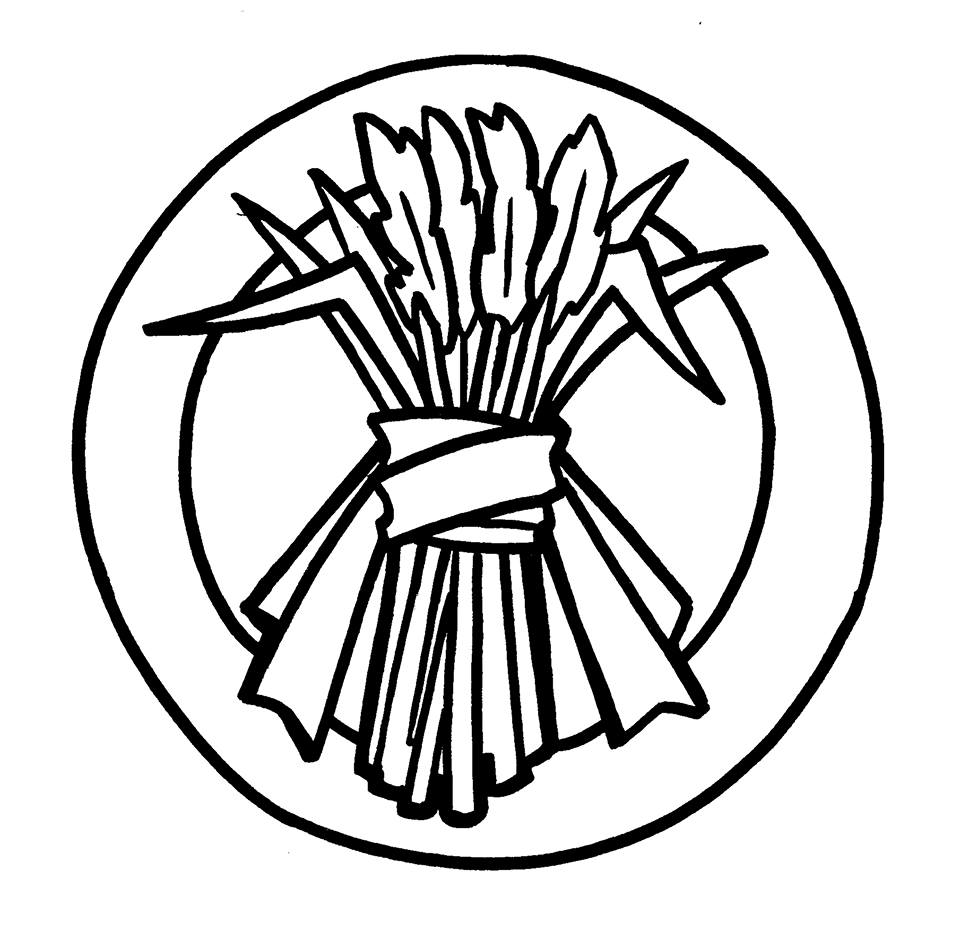
\includegraphics[width=5cm]{encyclopedia/StrongReeds}\caption{Strong reeds emblem}\end{figure}
\paragraph{Suaq} one of the three traditions of \s{Wintermark}
\paragraph{summer} 1: a season 2: the \s{magick}al realm of might and majesty
\paragraph{sutton quarries} a \s{white granite} quarry in \s{heath}, \s{Upwold}. an Imperial \s{bourse} position. The \s{jotun} have failed several times to claim the quarries.
\paragraph{synod} the governing body for matters of \s{faith}, where all priests with a congregation have voting rights.
\paragraph{taint} a wild growth of dangerous supernatural and exotic plants where a \s{briar} was buried.
\paragraph{tempest jade} a green stone, generally symbolised by a bolt of lightning. used for decoration and polishing by magicksmiths creating \s{magickal item}s. 
\paragraph{throne} 1: the constitutional body of the empress 2: the largest denomination of money, equivalent to 8 \s{crown}s or 160 \s{ring}s. a well-run farm makes a few thrones a year, and wains of \s{mithril}, \s{white granite} and \s{weirwood} are traded with thrones. \proverb{a pig on the throne with a crown on its head is still a ruddy pig.}
\paragraph{thule} the thule are inscrutable northern \s{orcs}, lead by \s{ritual}ists and fielding husks and fearsome beasts of war. coming from the resource-poor north, they are stripping dead enemies, invaded regions and captured territories of anything valuable. some of these resources are being used to reinforce their armies, but the lion's share is being sent north. fighting against the thule is fierce, especially since the disastrous death of empress \s{Britta} and most of her court. unlike other \s{barbarian}s, the thule do not make much use of subject tribes on the battlefield; rather they make extensive use of beasts, creatures, undead husks and spirits in their armies. The thule favour dark, hooded robes and cloaks, emphasizing their size and bulk with fur pelts over their shoulders. Thule consider a dark blue hue to be fortunate and revere dragons and wyrms as totemic beasts full of potence and cunning.\begin{figure*}\centering\includegraphics[width=8cm]{encyclopedia/Rhino}\caption{a thule war beast}\end{figure*}
\paragraph{Tom Drake} of Redston, legendary marcher general. In the first campaign of the \s{Empire}, Tom led his \s{household} and landskeepers from \s{Mitwold} to \s{varushka}. They fought through unfamiliar forests, alongside all those who opposed Alderei the fair and brought \s{varushka} into the \s{Empire}. some say it was Tom who killed the boyar-king; the Redston folk just point at the broken crown on their livery and let that speak for them. Tom Drake is also kent for his groundwork on the \s{constitution}al structure of the armies, and for his recipe of the Tom Drake's tea \s{potion}.
\paragraph{tower march} the region around \s{King's Stoke} in \s{Upwold}.
\paragraph{traumatic wound} any extraordinary type of \s{injury} that is not just a general loss of vitality due to blows with weapons including mortal wounds, or loss of function of limbs. a physick will be able to diagnose and right traumatic wounds.
\bigparagraph{trial} Trials settle disputes of law. They are presided over by a magistrate. it is their role to run trials in a manner which is expeditious and just. magistrates will aim to conclude trials within ten minutes in most circumstances and so time given to both witnesses and the accused will be strictly controlled. \localpar \keyword{Proceedings} The accused will be presented before the court by the militia. The accused may be accompanied by a priest (if they intend to plead guilty and ask for clemency) or possibly by a friend or legal advisor. The magistrate may choose to dismiss all the charges if they find no case to answer. otherwise, the charges against the accused will be detailed and they will then be asked how they plead in relation to each charge: guilty or not guilty. if the accused pleads guilty then before pronouncing punishment, the magistrate will allow any priest present (or the empress) to plead \s{clemency} on their behalf. alternatively, if a weregild arrangement has been made with the victim then this must be approved by the magistrate. \localpar The magistrate may also investigate and consider any other pertinent evidence or testimony prior to sentencing. if the accused pleads not guilty then the magistrate will make arrangements for a trial to be held to investigate the facts of the case to determine guilt. if the accused refuses to plea, then the magistrate may treat this as a guilty plea. in either case a plea for clemency will not be permitted. if all the relevant witnesses and evidence are available then the trial may proceed summarily. alternatively, if further investigations are required or witnesses are not currently available, the magistrate will release the accused on their oath that they will present themselves when it is time for their trial. occasionally a magistrate will set other limitations on the accused’s behaviour while awaiting trial. where a magistrate has reason to believe that the accused is an absconsion risk or will not comply with their conditions they may require the payment of monies or assets to the court in surety. these assets will be returned after the trial, provided that the accused does not abscond, breach any conditions or commit any further crimes. if an accused absconds then the magistrate may try them in their absence. it is likely the magistrate will draw an adverse inference from the accused's failure to attend and also find them guilty of contempt of court. any citizen can use reasonable force to apprehend them for the reward, although in practice it is often thief-takers and militia who are in the best position to do so. exceptionally, the magistrate may order the accused to be held in supervised custody until their trial can begin. this is only permitted where the magistrate believes the accused would be likely to commit further crimes if they were released. if so, the trial must be carried out as soon as reasonably practicable. the magistrate is responsible for investigating the facts of the case, not for acting as an impartial referee. if the magistrate is satisfied that the accused is unable to represent themselves adequately for some extraordinary reason then they may allow another person to speak in their stead. this does not exempt the accused from the requirement to answer any questions put to them by the magistrate. judgement is made by the presiding magistrate. occasionally a magistrate may ask one or more of their peers to sit with them in judgement over a particularly difficult case. the law allows magistrates to accept any evidence, including hearsay. the minimum persons required to be present for a trial to be valid are the presiding magistrate, and at least one other person. the accused should also be present if possible, but may be tried in their absence if they abscond. magistrates may choose to try all of those accused in connection with a particular crime or crimes at the same time. this is particularly likely where a criminal conspiracy by a group of individuals is suspected. where there are multiple offences which might apply to the accused the magistrate is only required to set out the most serious charge(s). this does not prevent the accused from being found guilty of a lesser related offence. if found guilty, the punishment will also take into account any relevant lesser offences where appropriate. when determining the accused's punishment the magistrate will take into account the seriousness of the crime and any mitigating factors, for example presented by a priest in their plea for clemency. \localpar \keyword{Clemency} when a person who is charged with a \s{crime} comes to the \s{trial} they have a choice—to plead guilty or not guilty. If, and only if, they plead guilty then they may ask for a priest (or the empress) to plead for clemency on grounds of \s{virtue} on their behalf. The magistrate reinholz has written a longer essay to aid priests provide a helpful plead for clemency. Normally the accused will have been given time before the trial to find a priest, to make their confession and to explain their actions, and to be \s{shriven}. No priest is obliged to make a plea for clemency. If the priest accepts this duty, they should take care to examine the facts of the case in detail. The priest must then use their own judgement of the \s{virtue}s of the act in question. They will be called as a witness to present a short plea for clemency to the court. Precisely how the priest deals with this is entirely up to the priest – indeed if the priest feels there is no virtue in the act then there is nothing wrong with the plea stating exactly that. If pleading clemency, priests should be aware that they will need to persuade the magistrate as to the virtues of the act in question. The magistrate is looking for facts which substantiate the defendanthe s actions as being virtuous. They are interested in the actual reasons in the mind of the defendant at the time of, and before the crime (rather than rationalisations afterwards). Talking about the motivation of the defendant may well help the plea by demonstrating the argument within the defendanthe s mind about the virtues of the act. Magistrates more likely to follow arguments which satisfactorily address the following sorts of issues: 1) why was due process unable to deal with the situation? 2) why did the burden fall upon this individual? 3) was the crime proportionate to the burden? \proverb{Every wife has two husbands and every husband two wives.}
\bigparagraphendtwiddle
\paragraph{trogoni} humanoid creatures with insect-like traits that live deep underground. they attack mana sites, consuming the mana crystals and feeding on the \s{magick}al flows. a single trogon is usually a match for an armoured warrior or two, with its tough carapace and savage rending claws.
\paragraph{tulpa} manifestation of a \s{constellation}. Tulpas are curious creatures – constructs of will and magick that make it easier to form a connection to a constellation. The process by which a tulpa forms and manifests is structurally and magically very similar indeed to the process by which an \s{egregore} is formed.
\paragraph{tusks} the fourth marcher army, made up from determined \s{Mournwold}ers. \proverb{war is a thrice-ploughed field.} \begin{figure}\centering\includegraphics[width=5cm]{encyclopedia/Tusks}\caption{Tusks emblem*}\end{figure}
\paragraph{Upwold} the easternmost marcher territory, fortified by the \s{eastern guard}. Unlike in \s{Mitwold}, a significant amount of Upwold's wealth comes from industries other than farming. While there are of course many farms in Upwold, the quick-growing silver birch woods on the eastern borders are the source of a great deal of income. Charcoal-burners live there, turning wood into easily transportable fuel for smith and hearth alike.
\paragraph{urizen} a \s{nation} of kenning magickians.
\paragraph{vallorn} the vallorn appeard when terunael, an \s{Empire} from \s{navarr}i prehistory, fell. from the hearts of their cities spread, a sick, infectious wave of life (\s{spring}) that crumbled stone, shot great trees up through streets and buildings, and warped what it found. around the core of each city areas of spring appeared, resistant to all efforts to destroy them. these were named vallorn. inside them are monstrous plants, the spores of which mutate living creatures that are exposed over many months. the air within the vallorn weakens those who enter, like venom. no complete catalogue exists – some things appear simply to be diseased, misshapen forest creatures, or mutated humans and orcs. some seem to be plants, sporting a mass of tangled thorns or possessing abilities that make them dangerous to travellers. a common threat to those who venture into those areas where the vallorn is strong are the vallornspawn husks (animated corpses). that being said, there are non-vallorn spring monstrosities like marshwalkers or trogoni. it is important to remember that they behave basically like animals: show no fear, back off slowly and calmly, don't offer violence, don't block exits, don't bring yourself to their attention if you can help it, and \emph{do not play dead}. climbing a tree may get you eaten by a tree.
\paragraph{varushka} a \s{nation} in the far north.
\paragraph{venom} many poisons (such as some \s{potion}s and the mists of the \s{druj} and \s{vallorn}) dilute the blood, making someone on the verge of death bleed out even faster. ways of alleviating this are listed in the essay on \s{medicine}.
\bigparagraph{vermin}\begin{figure*}\centering\includegraphics[width=\textwidth]{encyclopedia/vermin}\caption{types of vermin}\end{figure*}  \localpar \keyword{locusts} if you catch some of the locusts and burn them, the others will be stupefied by the smell. some will die, while others will fold their wings and wait to be caught, or will be killed by the sun. This arises from antipathy. Moreover, if you catch and burn a scorpion you will also catch the rest of the locusts, or drive them off. \localpar \keyword{weasels} they say that if one catches one of the weasels, cuts off its tail or testicles, and lets it go alive, one will not find any more of them afterwards on the same farm. \localpar \keyword{house mice} house mice are killed if you put down black hellebore with barley meal. They will also run away from copper sulphate, and the seeds of oregano, celery and love-in-a-mist burned as incense. you can also employ such means as help against rats. \localpar \keyword{field mice} some farmers in \s{Mitwold} have succeeded by blocking the holes with daffodils, so that as the field mice hurry to get out they will take the leaves with their teeth. When they bite them they will die. \localpar \keyword{foxes} a fox will not bite any bird under whose wing you have fastened wild rue. \localpar \keyword{snakes} no snakes will enter the farm if you plant wormwood or mugwort or southernwood around the farmstead; you will drive away those that are already there if you make smoke with white lily root or stag’s horn or goat’s hoof. Snakes will not trouble the pigeon-house if in its four corners you write “sentinel”. if it has windows, write it at these too. When a snake is going into its hole, if one catches its tail with the left hand one will easily pull it out again; if with the right hand it will be impossible to get it out. Either it will escape, or the tail will break off. \localpar \keyword{scorpions} if you rub your hands with radish juice, you can pick up scorpions and other such creatures without fear and without danger; and radishes, placed on scorpions, destroy them immediately. By frying a scorpion in olive oil and consecrating the place where someone has been stung by a scorpion you will alleviate the pain. \localpar \keyword{ants} if you catch and burn some ants you will drive away the rest of them, as experience has proved. If you spread cedar oil around their holes, ants will not come on the threshing floor. Ants will not attack a heap of grain if you draw round the heap with white earth, or put wild oregano around it. \localpar \keyword{mosquitoes} horsehair stretched across the door and through the interior of the house destroys mosquitoes and prevents them from entering. If you soak a sponge in sharp vinegar and hang it at your head and at your feet when in bed, the mosquitoes will not bite you. \localpar \keyword{bats} if you hang plane leaves in their path, they will not approach. Smoked ivy kills bats. \localpar \keyword{fleas} in the house, dig a hole; grind oleander leaves and place in it; they will all gather there. Otherwise, soak the floor repeatedly with amorge; then grind wild cumin and mix with waters, and grind 10 drams of squirting cucumber seed and add to the water; sprinkle this in the room and you will make the fleas split. \localpar \keyword{leeches} if an ox or other quadruped swallows a leech while drinking, squash some bugs, let the animal smell them and it will immediately eject the leech. \localpar \keyword{frogs} frogs will stop their croaking if you light a candle and put it on the river-bank. \localpar \keyword{rats} rats reproduce quicker than any other animal, and harm your corn, bacon, cheese and other provisions. Fortunately, the natural enemies of rodents can be employed, by having a good array of cats. A cat corpse with a dead mouse stuffed in their mouth is sometimes built into the foundations of a house as it deters other rodents from entering the premises. To catch rats, rat-catchers employ traps made of little planks upon sticks or poisoned bait of an ounce of aconite, two ounces of fine arsenic, a quarter of pig's fat, a pound of fine wheaten meal and four eggs, made into a bread and cooked in the oven and cut into strips; or cakes of paste and powdered aconite, setting these near to their holes where they have naught to drink; or black hellebore mixed with fat, bread, cheese or flour; or the juice of bruised wild cucumber, which slays the mice as diverse men have said. \localpar \s{boggart}s simple traps can catch \s{boggart}s, and regular checking of dark corners for boggart eggs helps rout an infestation. \bigparagraphendtwiddle
\paragraph{Vigilance} a \s{virtue} \proverb{A man warned a man is half saved.}
\paragraph{virtue} the \s{faith} of the way is composed of the seven virtues \s{Loyalty}, \s{Vigilance}, \s{Ambition}, \s{Courage}, \s{Pride}, \s{Wisdom}, and \s{Prosperity}, and Imperial priests can perform ceremonies that actualise these virtues in the world. Individuals following the virtues transit through the \s{labyrinth} faster and can ultimately leave it behind and become \s{paragon}s. False virtues, such as hope, \s{fear} or peace, try to steer honest \s{citizen}s away from the way. \proverb{Ambition, Prosperity, Loyalty, Pride – Empire strong and the foe outside\\Courage and Wisdom, and Vigilance true – Empire's future depends upon you.}
\paragraph{wassail} after every harvest, Marcher farmers perform this traditional religious ceremony to celebrate Prosperity. Wassailing varies from place to place but typically involves parading through the village singing and drinking to the health of the fields and orchards. Food and drink produced during the year is consumed or left as an offering; ale might be used to toast a barley field or a pat of butter buried in a dairy pasture. The parade is often led by the children of the village. As the yeomen go from house to house they share food and drink with their community and receive in return a taste of the food that each \s{household} has in excess from their own harvests. At each autumn equinox, Marchers parade from camp to camp, singing the wassail and sharing their home-grown produce with other \s{nation}s. Although not expected, other nations often reciprocate in small token exchanges of goods that their own territories have in abundance.
\paragraph{Wayford} A large \s{market town} and monastery at the confluence of the upper tributaries of the Meade. A layer of gritstone in between the chalk of the wolds means the river is wide and shallow, allowing livestock from the hills to cross, or embark on riverboats to Meade itself. At the river fork in Wayford stand several gibbets with a long and bloody history, notable in recent years for playing host to Red Walder and his outlaws, a plague on the \s{Mitwold} for many years. The town is also notable due to legends that \s{Jack-in-chains} is buried somewhere nearby.
\paragraph{weakness} an affliction of the body, see the treatise on \s{medicine}.
\paragraph{wendigo} \keyword{harvester of graves}, \keyword{abominable one}. The worst \s{winter} \s{eternal} kent to the Empire. Stories suggest that food eaten or drink drunk will cause a stomach upset while you still have the same saliva in your mouth that spoke his name or any of his epithets. He has been under \s{enmity} since 306 YE, because he tempts Imperial citizens to ritual murder, cannibalism, \s{heresy}, \s{blasphemy} and \s{idolatry}.
\paragraph{weirwood} one of the four strategical Imperial resources, distributed by the bourse. Weirwood is used to improve farms, herb gardens and ships, and to supply armies or repair fortifications.
\paragraph{weltsilver} a slightly tinted silver metal, generally symbolised by a blood droplet. Used by magicksmiths to create jewellery or \s{magickal item}s that channel energy.\begin{figure}\centering\includegraphics[width=4cm]{encyclopedia/weltsilver}\caption{weltsilver}\end{figure} 
\paragraph{Westmere} a large lake north of the Marches, between \s{Bregasland}, \s{Mitwold} and Kallavesa in \s{Wintermark}. It connects to the Gullet to the west, and from there to the oceans.
\paragraph{whisper-gallery} a collection of \s{herald}s or \s{eternal}s of \s{night}, obsessed with secrets. Their heralds, kent as sommeliers, look like retainers, clothed in white and wearing mask and gloves. The individual courtiers appear in robes, masks and gloves of different colour and have different interests. Unlike some other \s{night} \s{eternal}s, they are equally concerned with learning secrets and with ensuring that secrets remain secrets. They have also evidenced some interest in the way that the things individuals believe they ken about each other influence their interactions and desires.
\paragraph{white granite} one of the four strategical Imperial resources, distributed by the bourse. White granite is used to improve forests, churches and businesses, and to create or repair fortifications.
\paragraph{wicker man} this is a large figure of wicker and wood, which is set alight to burn sacrifices at \s{wassail}. Ideal sacrifices are things that have been raised by mortal hands from the land such as crops and domesticated animals. These sacrifices are made to atone for \s{sin}s. By giving up the rewards of \s{Prosperity}, and creating the need for more Prosperity to replace them, the Marchers believe that they make reparation for their unvirtuous behaviour and in this way ensure that they reincarnate well in the next life. The greatest sacrifice of all is to give up ones own life. This is only ever permitted for individuals whose failure cannot otherwise be redeemed. By going voluntarily to the wickerman they absolve not just their own failure but the failures of everyone who served under them. The most recent example was in 349 when former senator Thomas Overton of the \s{Mournwold} went into the wicker man to absolve himself for his inability to keep his territory out of jotun hands. Similarly to the wicker man, many Marchers burn their poppets at wassail to atone for small \s{sin}s and transgessions. 
\paragraph{willot'wisp} an atmospheric ghost light seen by travellers at night, especially over bogs, swamps or marshes in \s{Bregasland}. It resembles a flickering lamp and is said to recede if approached, drawing travellers from the safe paths.
\paragraph{winter} 1: a season 2: the \s{magick}al realm of cruelty and choices
\paragraph{Wintermark} a \s{nation} of there different people north of the Marches. The inhabitants of the Mark are the Kallavesi, the Suaq and the Steinr, the three traditions of Winterfolk.
\paragraph{Wisdom} one of the seven \s{virtue}s. Wisdom is the path of being aware of your ken, but also its boundaries and how to extend them. \proverb{Having a grey beard doesn’t make you wise.}
\paragraph{wound} \see{injury}
\paragraph{yeoman} a farmer who owns the land they toil
\paragraph{yeomen} \see{yeoman}
%%% Local Variables: 
%%% TeX-engine: xetex
%%% TeX-master: "encyclopedia"
%%% coding: utf-8
%%% mode: latex
%%% End: 


% constellation?
% conclave order
% grandmaster
% sodality
% Green Men and Jacks

% Add insets
% Add songs

